 \documentclass[10pt,a4paper]{book}
        
\usepackage{amssymb}% for numbers/numbers
\usepackage{lscape}

\usepackage{sectsty}
\allsectionsfont{\sffamily}

\setlength{\textheight}{24cm}
\setlength{\textwidth}{15.912cm}

\setlength{\evensidemargin}{0cm}
\setlength{\oddsidemargin}{0cm}

\setlength{\topmargin}{-0.5cm}
%\setlength{\parindent}{0cm}


\usepackage{listings}
\usepackage{color}
\lstdefinestyle{defaultstyle}{}
\lstset{language=Python}
\lstset{basicstyle=\ttfamily}
\lstset{showstringspaces=fales}
\lstset{keywordstyle=\color{blue}}
\lstset{frame=single}
%\lstset{backgroundcolor=\color{white},emph={EMPTY},emphstyle=\color{white}}
%\definecolor{lightgrey}{cmyk}{0.1,0.1,0.1,0}
%\lstset{backgroundcolor=\color{lightgrey}}

\renewcommand{\labelitemii}{\ensuremath{\triangleright}}    %  open triangle replaces default dash

\newcommand{\py}[1]{\texttt{\color{blue}#1}}

\newcommand{\nmesh}{\texttt{nmesh}}
\renewcommand{\nsim}{\texttt{nsim}}
\newcommand{\nsimi}{\texttt{nsim\_i}}



\usepackage{graphicx}

\usepackage[dvips=true,bookmarks=true]{hyperref} 


\begin{document} 



\title{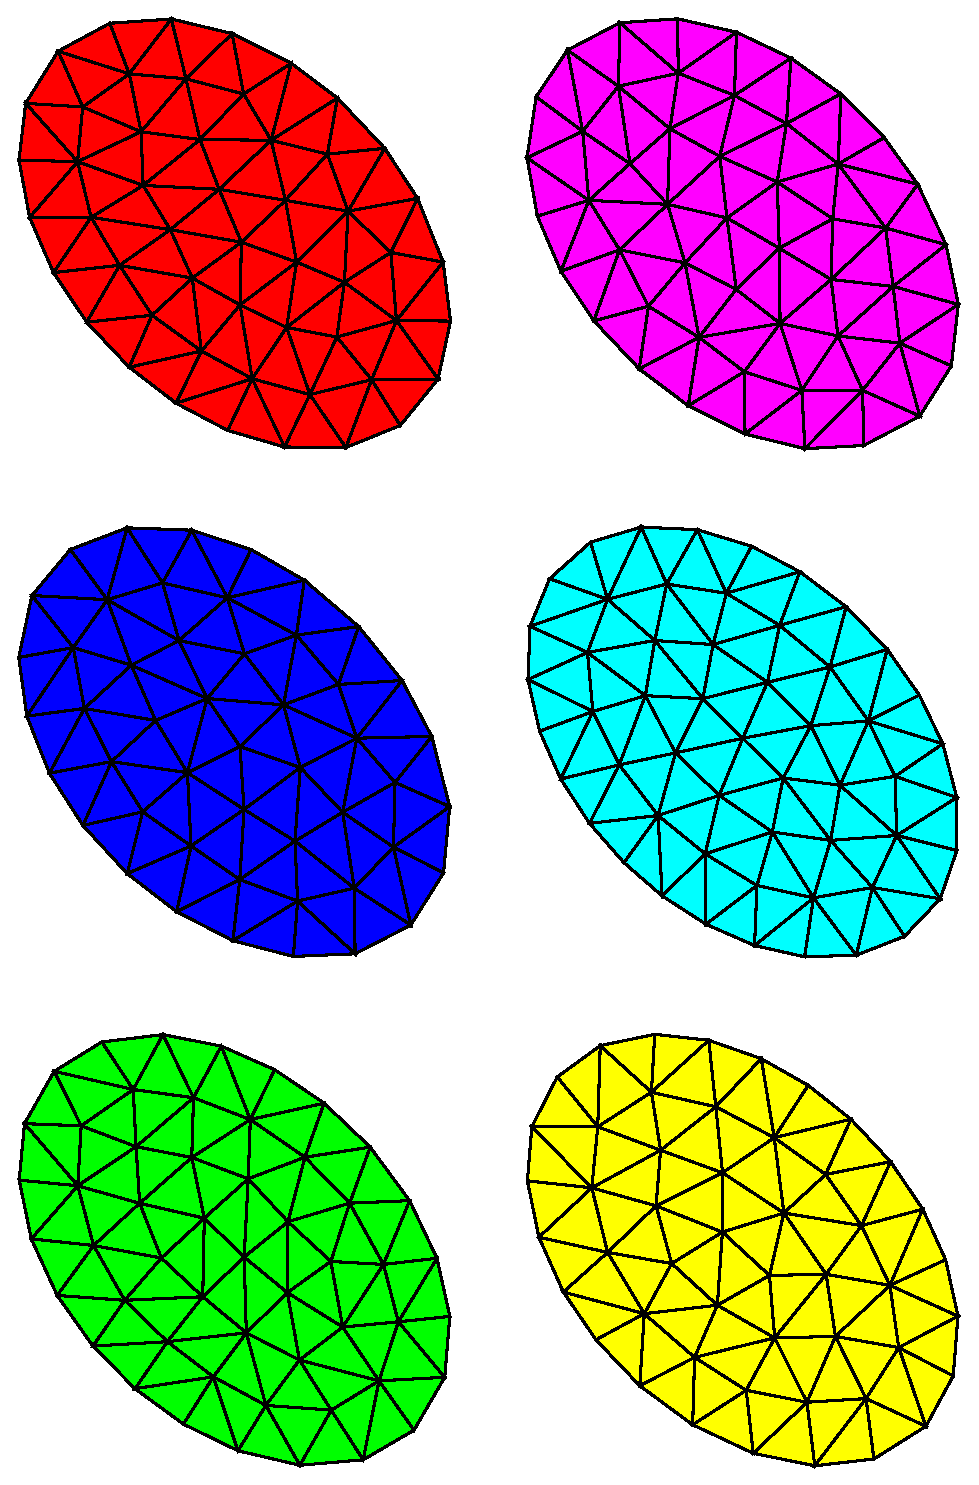
\includegraphics[width=5cm]{plots/somemesh}\\[2cm] 
\sffamily \huge nmesh --- user manual\thanks{ \sffamily \footnotesize $ $Id$ $}
}
\author{ \sffamily University of Southampton\\
\sffamily Thomas Fischbacher, Giuliano Bordignon, Matteo Franchin, Hans Fangohr\\}

\date{\small \sffamily $ $Date$ $ }

\maketitle


\chapter*{Acknowledgements}

\begin{itemize}
\item This work has (partly) been funded by EPSRC.
\item We thank Jacek Generowicz and Marc Molinari for their input at the
very early stages of this project. 
\item James Kenny has contributed routines for the visualisation of the meshes. 
\item Kondwani Kanjere has
contributed to finding optimal meshing parameters (in two dimensions),
\end{itemize}

\tableofcontents
\chapter{Introduction}

The approach used to create the mesh is based on the method proposed
by Persson and Strang \\
(cf. \texttt{http://www-math.mit.edu/\~persson/mesh/})
where an initial set of points is distributed randomly over the region
to be meshed. Every point is then connected to its nearest neighbours,
and a force acting along the connection push them apart with a linear
force. The relaxation proceeds until an equilibrium of forces or a
predefined number of iterations is reached.  

Some new techniques have been added to improve the mesh quality.

The code is implemented in a compiled language.

\section{Warning: Alpha release}
\label{sec:release}

The code is relatively new. As a result, a number of bugs can be
expected in the program. It is also possible that we realise design
errors and that names of functions, or their signature may change in
future.




%\chapter{Installation}
%--to be addressed --; possibly in another file

\chapter{Quick start}

\section{Introduction}
To create a mesh, we need to write a Python script that contains the
geometry information of the objects that are do to be meshed. In this
chapter, we provide and explain a number of simple examples.

\section{Meshing one object}

\subsection{Meshing an ellipsoid (\texttt{tutorial1.py}) }
\label{sec:meshing-an-ellipsoid}

\lstinputlisting[numbers=left]{../examples/tutorial1.py}

Line 1 imports the \py{nmesh} module. All our meshing scripts have to
start with this line.

Line 3 creates a first ``object'' that we would like to mesh. In this
case it is an \py{ellipsoid}, and the ellipsoid is provided by the
nmesh-packages (therefore we have to access it with
\py{nmesh.ellipsoid}. We pass two parameters to the ellipsoid, and this are the semi-axes in x-, and y- direction for the ellipsoid.

Note that at this point we have decided to create a two-dimensional mesh. Had we created an ellipsoid object like this,
\begin{lstlisting}
cigar = nmesh.ellipsoid( [4,2,5] )
\end{lstlisting}
the we would have a \emph{three-dimensional} object because we have specified the lengths of \emph{three} semi-axes for the ellipsoid.

Line 5 defines a bounding box. The bounding box is a cuboid defined by providing the positions of opposite corners. It is always necessary to provide a bounding box that encloses all the objects to be meshed. See also \ref{sec:boundingbox}.

Line 7 carries out the actually meshing work. The arguments given to the function \py{nmesh.mesh()} are (in this simple case) a list of objects that we would like to mesh. Since we only want to mesh the \py{cigar}, we include only the cigar in this object list. The function returns a ``mesh-object''.

Line 9 creates a postscript file that visualises this mesh, and saves this postscript file to a file with name ``\texttt{tutorial1.ps}''.

If we run this script, it produces a mesh similar to the one shown in figure \ref{fig:tutorial1}.

\begin{figure}[tbh]
\centerline{\includegraphics[width=0.3\textwidth]{figures/tutorial1}}
\caption{\label{fig:tutorial1}The output of the \py{tutorial1.py} example.}
\end{figure}



\section{The bounding box}
\label{sec:boundingbox}
The surfaces of objects are internally defined as positions in space
where certain geometry functions take values of zero. It is therefore
necessary to tell the mesher where in real space these roots of those
functions are located and this is done by providing the bounding box.

The bounding box can either be meshed as well (in which case
\py{mesh\_bounding\_box} has to be set to true, see
\ref{sec:meshingtheboundingbox}) or remain unmeshed (this is the
default).

However, the bounding box has to be provided. If the bounding box is
chosen too small, then elements that are outside the bounding box may
not be meshed correctly. If the bounding box is chosen too large, this
doesn't affect the final mesh but it slows down the meshing process.

\section{Meshing objects and the exterior}

\subsection{Meshing the bounding box (\texttt{tutorial2.py})}
\label{sec:meshingtheboundingbox}

\lstinputlisting[numbers=left]{../examples/tutorial2.py}

In this example, we have embedded the cigar in a meshed outer space
(what is called the ``bounding box''). This is done by defining the
bounding box as shown in line 5. The bounding box is given as a pair
of points in space that span the bounding box. In this case, one of
the corners of the box is at $(-5,-5)$ and the other one is at
$(5,5)$. 

To mesh the outer space, we have to provide the
\py{mesh\_bounding\_box=True} argument to \py{nmesh.mesh()} as shown
above in line 8.


If we run this script, it produces a mesh similar to the one shown in figure \ref{fig:tutorial2}.

\begin{figure}[tbh]
\centerline{\includegraphics[width=0.3\textwidth]{figures/tutorial2}}
\caption{\label{fig:tutorial2}The output of the \py{tutorial2.py} example.}
\end{figure}


 
\subsection{Changing the  (uniform) node density (\texttt{tutorial3.py})}

\lstinputlisting[numbers=left]{../examples/tutorial3.py}

In this example (see figure \ref{fig:tutorial3}), we have increased the node density by a factor of 4 (in comparison to figure {fig:tutorial2}). 

The only change (in comparison to \texttt{tutorial2}) is the addition
of \py{a0=0.5} to line 7.

We need to know a bit more about the default assumptions of the
mesher. If no node density is provided, the mesher will generate as
many nodes as required to obtain a density of one node per unit
volume.\footnote{This is to read as the n-dimensional volume; \emph{i.e.} for
our two-dimensional examples the two-dimensional volume is what is
ofter referred to as area}

The mesher will work out what the required edge length is to achieve
this density. We can modify the density by asking the mesher to
multiply this edge length with a number \py{a0}. The default of
\py{a0} is 1.0. In this example, we have changed it to 0.5, and
therefore we have increased the node density by a factor of 4 (because
we are two dimensions).

This script produces a mesh similar to the one shown in figure
\ref{fig:tutorial3}.

\begin{figure}[tbh]
\centerline{\includegraphics[width=0.3\textwidth]{figures/tutorial3}}
\caption{\label{fig:tutorial3}The output of  the \py{tutorial3.py} example.}
\end{figure}


\section{The fundamental objects}
\label{sec:fundamentalobjects}

\subsection{The ellipsoid}
We have already seen an example for an ellipsoid in section \ref{sec:meshing-an-ellipsoid}. As mentioned before, higher-dimensional ellipsoids are created by providing more lengths for the semi-axes (one for each dimension).
\subsection{The box}

\lstinputlisting[numbers=left]{../examples/box.py}

A box is an n-dimensional cuboid and defined by providing the spatial coordinates of two opposite corners. In the example above, these corners are [0,0] and [5,10]. Note that each corner point must be provided as a python list, and both corners need to be provided within another list (as shown in \texttt{tutorial3.py} above. This script produces a mesh similar to the one shown in figure \ref{fig:box}.

\begin{figure}[tbh]
\centerline{\includegraphics[width=0.3\textwidth]{figures/box}}
\caption{\label{fig:box}The output of  the \py{box.py} example.}
\end{figure}


\subsection{The conical frustum}
\begin{figure}[tbhp]
\centerline{\includegraphics[width=0.3\textwidth]{plots/frustum3d}}
\caption{\label{fig:frustum3dsketch} The points P1 and P2 and the radii R1 and R2 of the circles around P1 and P2 are used to define the frustum.}
\end{figure}
Figure \ref{fig:frustum3dsketch} shows how the frustum is defined in the following example:
\lstinputlisting{../examples/frustum.py}
The output of this script is shown in figure \ref{fig:frustum}.
\begin{figure}[tbhp]
\centerline{\includegraphics[width=0.3\textwidth]{figures/frustum}}
\caption{\label{fig:frustum}The output of the \py{frustum.py} example. In two dimensions, the frustum appears as a trapezoid.}
\end{figure}




\subsection{The conical frustum in three dimensions}
All of the objects listed here can be meshed in any (positive-integer) number of dimensions (see also section \ref{sec:meshing-n-dimensions}). We show only the frustum as 3d object to demonstrate this.

\lstinputlisting{../examples/frustum3d.py}
The output of this script is shown in figure \ref{fig:frustum3d}.
\begin{figure}[tbhp]
\centerline{\includegraphics[width=0.3\textwidth]{figures/frustum3d}}
\caption{\label{fig:frustum3d}The output of the \py{frustum3d.py} example.}
\end{figure}




\section{Translating, scaling and rotating objects}


All mesh objects can be translated (``shift''), scaled and rotated.
This section provides some examples.



\subsection{Translation (\texttt{shift.py})}
\label{subsec:shifting}

The easiest transformation is to translate an object. This is done by adding an optional argument with name \py{transform} to the constructor of the object. For example, to shift a box with unit volume by 3 units in x and 4 units in y (in two dimensions), we could use this line:
\begin{lstlisting}
box = nmesh.box( [0,0],[1,1], transform=[ ("shift",[3,4]) ] )
\end{lstlisting}
Note that actual shift transformation is just \py{("shift",[3,4])}. The first argument of the tuple specifies that we request a \py{shift}, the second argument is the translation vector.

Because many such transformations can be specified, these are accumulated in a list (that's where the square brackets come from).

Here is a complete example:
\lstinputlisting{../examples/shift.py}
and figure \ref{fig:shift} shows the output.
\begin{figure}[tbhp]
\centerline{\includegraphics[width=0.3\textwidth]{figures/shift}}
\caption{\label{fig:shift} The output of the \py{shift.py} example.}
\end{figure}


\subsection{Scaling (\texttt{scale.py})}

The syntax for scaling is very similar to the syntax for shifting (\ref{subsec:shifting}). Here is an example
\lstinputlisting{../examples/scale.py}
and figure \ref{fig:scale} shows the corresponding mesh.
\begin{figure}[tbhp]
\centerline{\includegraphics[width=0.3\textwidth]{figures/scale}}
\caption{\label{fig:scale} The output of the \py{scale.py} example.}
\end{figure}


\subsection{Rotation}


\subsubsection{In 2 dimensions (\texttt{rotate2d.py})}

Rotation in 2d requires only one angle (in degree). The rotation is carried out in the mathematical sense (i.e. counter clock wise). Here is an example
\lstinputlisting{../examples/rotate2d.py}
and figure \ref{fig:rotate2d} shows the corresponding mesh.
\begin{figure}[tbhp]
\centerline{\includegraphics[width=0.3\textwidth]{figures/rotate2d}}
\caption{\label{fig:rotate2d} The output of the \py{rotate2d.py} example.}
\end{figure}

\subsubsection{In 3 dimensions (\texttt{rotate3d.py})}
In three dimensions there is a transformation with name \py{rotate3d}
which accepts an axis to rotate around and an angle (in degree)
specifying how far to rotate around that axis.

The transformation to rotate around [0,0,1] for 45 degrees would thus read
\begin{lstlisting}
("rotate3d",[0,0,1],45)
\end{lstlisting}
The complete example is
\lstinputlisting{../examples/rotate3d.py} 
and creates the mesh shown in figure~\ref{fig:rotate3d}.
\begin{figure}[tbhp]
\centerline{\includegraphics[width=0.3\textwidth]{figures/rotate3d}}
\caption{\label{fig:rotate3d} The output of the \py{rotate3d.py} example.}
\end{figure}


%where the use of the \py{visual} module allows to 
%visualise the 3D mesh in MayaVi, as explained in Chapter
%\ref{chap.visual_module}.  

\subsubsection{In $n$ dimensions (\texttt{rotate.py})}
In general, a rotation is carried out by specifying the indices of the
dimensions around which no rotation takes place, and an angle. The syntax to rotate 45 degrees in the x-y plane would therefore be
\begin{lstlisting}
("rotate",[0,1],45)
\end{lstlisting}
Here is the example of a rotation around the \textit{z}-axis:
\lstinputlisting{../examples/rotate.py} 
and figure \ref{fig:rotate} shows the corresponding mesh.
\begin{figure}[tbhp]
\centerline{\includegraphics[width=0.3\textwidth]{figures/rotate}}
\caption{\label{fig:rotate} The output of the \py{rotate.py} example.}
\end{figure}
\subsection{Combining transformations (\texttt{transformations})}

Any number of transformations can be specified in a list, and are
carried out in the order they are given in the list.

Here is a more complex example
\lstinputlisting{../examples/transformations.py}
and figure \ref{fig:transformations} shows the corresponding mesh.
\begin{figure}[tbhp]
\centerline{\includegraphics[width=0.3\textwidth]{figures/transformations}}
\caption{\label{fig:transformations} The output of the \py{transformations.py} example.}
\end{figure}

\section{Combining objects}
\label{sec:combiningobjects}
In most applications, we would like to mesh more complicated systems,
consisting of more than one fundamental geometry type. We have a
number of options how to combine these within \nmesh.

\subsection{Plotting several objects (\texttt{multiobjects.py})}
\label{sec:multiobjects}

We can simply create more objects and mesh these together by providing
them in a list to \py{nmesh.mesh()}. Here is an example
\lstinputlisting{../examples/multiobjects.py}
and figure \ref{fig:scale} shows the corresponding mesh.
\begin{figure}[tbhp]
\centerline{\includegraphics[width=0.3\textwidth]{figures/multiobjects}}
\caption{\label{fig:multiobjects} The output of the \py{multiobjects.py} example.}
\end{figure}

\subsection{Union (\texttt{union.py})}
\begin{lstlisting}
union = nmesh.union([A,B,C,D])
\end{lstlisting}
The \py{nmesh.union()} function takes a list of objects (here A,B,C and D) and returns an object that is the union of the provided objects. The list of objects can be of any length. 

This allows to ``merge'' several objects together. Here is an example:
\lstinputlisting{../examples/union.py}
and figure \ref{fig:scale} shows the corresponding mesh.
\begin{figure}[tbhp]
\centerline{\includegraphics[width=0.3\textwidth]{figures/union}}
\caption{\label{fig:union} The output of the \py{union.py} example. A circle and a rectangle are merged together.}
\end{figure}


\subsection{Difference (\texttt{difference.py})}
To ``subtract'' one objects from another, one can use the \py{nmesh.difference()} function. Its syntax is:
\begin{lstlisting}
diff = nmesh.difference(A,[B,C,D])
\end{lstlisting}
This would subtract objects B,C and D from object A, and return the new difference object.
Here is a complete example
\lstinputlisting{../examples/difference.py}
and figure \ref{fig:scale} shows the corresponding mesh.
\begin{figure}[tbhp]
\centerline{\includegraphics[width=0.3\textwidth]{figures/difference}}
\caption{\label{fig:difference} The output of the \py{difference.py} example. A small ellipse is removed from a large ellipse, leaving an ``elliptical ring''.}
\end{figure}

\subsection{Intersection (\texttt{intersection.py})} 
\begin{lstlisting}
intersection = nmesh.intersection([A,B,C,D])
\end{lstlisting}
The \py{nmesh.intersection()} function takes a list of objects (here A,B,C and D) and returns an object that is the intersection of the provided objects. The list of objects can be of any length. Here is an example:
\lstinputlisting{../examples/intersection.py}
and figure \ref{fig:intersection} shows the corresponding mesh.
\begin{figure}[tbhp]
\centerline{\includegraphics[width=0.3\textwidth]{figures/intersection}}
\caption{\label{fig:intersection} The output of the \py{intersection.py} example showing the intersection of an ellipsoid and a cone.}
\end{figure}



\section{Saving and loading meshes (\texttt{save\_load.py})}
\label{sec:saveload}

Once a mesh object \py{mesh} has been created, it can be saved using the
\py{mesh.save(FILENAME)} command. The file extension \py{.nmesh} is
recommended for mesh data files (but not required).

This code shown below
\begin{itemize}
\item creates a mesh
\item saves it to the file \texttt{save\_load.nmesh}
\item loads it from the file \texttt{save\_load.nmesh}
\item and creates a postscript plot (shown in figure \ref{fig:saveload}).
\end{itemize}
\lstinputlisting{../examples/save_load.py}
\begin{figure}[tbhp]
\centerline{\includegraphics[width=0.3\textwidth]{figures/save_load}}
\caption{\label{fig:saveload} The output of the \py{save\_load.py} example.}\end{figure}


\section{Meshing in $n$-dimensions}
\label{sec:meshing-n-dimensions}

With the exception of the visualisation routines, \nmesh{} is able to
generate meshes in any number of dimensions. The number of dimensions
is defined implicitely by providing $n$-dimensional points to object constructors. We demonstrate this for an ellipsoid.

\subsection{1d ellipsoid (\texttt{simple1d.py})}

This is a trivial example:
\lstinputlisting{../examples/simple1d.py}

We request a one-dimensional ellipsoid with semi-axis length 1.0. The object is one-dimensional because we provide only one length for the semi-axes. In other words, we should get an 'object' with boundaries at +1.0 and -1.0. 

We mesh the surrounding space up to +2 and -2 because these are the limits of the one-dimensional bounding box. 

After computing the mesh, we obtain an output file (\texttt{simple1d.nmesh}) which starting in line 3 contains the positions of the nodes of the 1d mesh:
\lstinputlisting[firstline=1,lastline=12,basicstyle=\ttfamily\footnotesize]{figures/simple1d.nmesh}

% %FIX ME XXX KKK Need to updaet this in the end. %%% We see that indeed there are nodes on the 'surface' of the ellipsoid (at approximately +1 and -1), and at the boundary of the boundary box (+2 and -1). The interior of the ellipsoid contains further nodes at approximately 1/3 and -1/3.\footnote{The requested density was 1.0, so that we don't expect any extra nodes between 1.0 and 2.0. The interior of the ellipsoid has a higher density (because there are three nodes over a volume of 2, so it is 1.5) because the meshers needs to put some 'tension' into the system by using some more nodes than necessary to obtain the ideal density.}


\subsection{2d ellipsoid (\texttt{simple2d.py})}

This is the 2d example 
\lstinputlisting{../examples/simple2d.py}
and produces the mesh shown in figure \ref{fig:simple2d}
\begin{figure}[tbhp]
\centerline{\includegraphics[width=0.3\textwidth]{figures/simple2d}}
\caption{\label{fig:simple2d} The output of \py{simple2d.py}.}
\end{figure}


\subsection{3d ellipsoid (\texttt{simple3d.py})}

This is the 3d example 
\lstinputlisting{../examples/simple3d.py}
and produces the mesh shown in figure {fig:simple3d}
\begin{figure}[tbhp]
\centerline{\includegraphics[width=0.3\textwidth]{figures/simple3d}}
\caption{\label{fig:simple3d} The output of \py{simple3d.py}.}
\end{figure}


\subsection{4d ellipsoid (\texttt{simple4d.py})}

This is the 4d example 
\lstinputlisting[lastline=10]{../examples/simple4d.py}
The mesh of the 4d ellipsoid is difficult to plot. We show in figure \ref{fig:simple4d} \emph{projections} of the 4d-positions of the nodes into some two-dimensional subspaces defined by two of the four coordinates being 0.

If we project the positions of a 3d sphere into two dimensions (for example by ``ignoring'' the $z$-component and plotting all nodes in the $x$-$y$-plane, we expect to obtain a circle filled with the nodes.

Similar arguments show that by projecting a 4d ellipsoid in two
dimensional subspaces we expect filled ellipsoids. Comparison of the
semi-axis of the 2d projections in figure \ref{fig:simple4d} with the
command to create a 4d ellipsoid with the semi-axes defined in
\texttt{simple4d.py} shows that the ellipsoid has the expected shape.

\begin{figure}[p]
\begin{tabular}{p{2cm}c}
\parbox{2cm}{Projected into dimensions 0 and 1}& \parbox{0.8\textwidth}{\includegraphics[width=0.8\textwidth]{figures/simple4d_proj01}}\\
%\parbox{2cm}{Projected into dimensions 1 and 2}& \parbox{0.8\textwidth}{\includegraphics[width=0.8\textwidth]{figures/simple4d_proj12}}\\
\parbox{2cm}{Projected into dimensions 2 and 3}& \parbox{0.8\textwidth}{\includegraphics[width=0.8\textwidth]{figures/simple4d_proj23}}\\
%\parbox{2cm}{Projected into dimensions 3 and 0}& \parbox{0.8\textwidth}{\includegraphics[width=0.8\textwidth]{figures/simple4d_proj30}}\\
\end{tabular}
\caption{\label{fig:simple4d} Projections of the 4-dimensional positions of the nodes into two dimensionsal subspaces.}
\end{figure}



\chapter{More  examples (gallery)}


\section{Arrays of objects}

\subsection{Ellipsoids (\texttt{ellipsoid\_array.py})}

This code 
\lstinputlisting{../examples/ellipsoid_array.py}
computes the mesh shown in figure \ref{fig:ellipsoidarray}.
\begin{figure}[tbhp]
\centerline{\includegraphics[width=0.3\textwidth]{figures/ellipsoid_array}}
\caption{\label{fig:ellipsoidarray} The output of the \py{ellipsoid\_array.py} example showing an array of ellipsoids.}
\end{figure}

\subsection{Ellipsoids (3d) (\texttt{ellipsoid\_array3d.py})}

This code 
\lstinputlisting{../examples/ellipsoid_array3d.py}
computes the mesh shown in figure \ref{fig:ellipsoidarray3d}.
\begin{figure}[tbhp]
\centerline{\includegraphics[width=0.5\textwidth]{figures/ellipsoid_array3d}}
\caption{\label{fig:ellipsoidarray3d} The output of the \py{ellipsoid\_array3d.py} example showing an array of ellipsoids in three dimensions.}
\end{figure}


\subsection{Merged sphere array (\texttt{mergedspheres.py})}

This code 
\lstinputlisting{../examples/mergedspheres.py}
computes the mesh shown in figure \ref{fig:mergedspheres}.
\begin{figure}[tbhp]
\centerline{\includegraphics[width=0.3\textwidth]{figures/mergedspheres}}
\caption{\label{fig:mergedspheres} The output of the \py{mergedspheres.py} example.}
\end{figure}



\section{Periodic meshes (\texttt{periodic.py)}}
\label{sec:periodicmeshes}

For periodic meshes, it is required to specify a boolean vector and
the bounding box. The default value of the vector elements is False, which
correspond to non-periodic meshes, and the periodicity is defined
axis-wise setting to True the element corresponding to the specific axis. 
Here is an example 
\lstinputlisting{../examples/periodic.py}
computes the mesh shown in figure \ref{fig:periodic}.
\begin{figure}[tbhp]
\centerline{\includegraphics[width=0.3\textwidth]{figures/periodic}}
\caption{\label{fig:periodic} The output of the \py{periodic.py} example.}
\end{figure}



\section{Spatially varying density}


If required, the node density can be provided as a function of space.
To do this, the user needs to write a short C-program that computes
the density, given a position in space.

The position in space is provided in the array \py{x}. Index 0
corresponds to the first spatial dimension, index 1 to the second and
so on. The C-Program needs to store the resulting density an a
variable called \py{density}. 

Here is an example, to have a density that increases in $x$-direction with a slope of 2 and in $y$-direction with a slope of 4, we could use this C-Program:
\begin{lstlisting}
density = 1.0 + x[0]*2.0 + x[1]*4.0;
\end{lstlisting}
We can introduce our own variables if we like, and write
\begin{lstlisting}
double xslope = 2.0;
double yslope = 4.0;
density = 1.0 + x[0]*xslope + x[1]*yslope;
\end{lstlisting}

To pass the C-programme to the mesher, we have to store in a string, and give the string to the \py{nmesh.mesh()} command as an argument with name \py{density}. 

\subsection{Simple example (\texttt{density1.py})}

Here is a complete example where the density increases in $y$-direction:
\lstinputlisting{../examples/density1.py}
computes the mesh shown in figure \ref{fig:density1}.
\begin{figure}[tbhp]
\centerline{\includegraphics[width=0.3\textwidth]{figures/density1}}
\caption{\label{fig:density1} The output of the \py{density1.py} example.}
\end{figure}

\subsection{More complex example (\texttt{density2.py})}

Here is a more complicated example. Note that if we provide a scaling factor \py{a0} for the edge length, than the density will be multiplied with ${a_0}^{1/d}$ where $d$ is the number of dimensions. The parameter \py{a0} provides the possibility to simply change the edge length globally (and defaults to 1.0).
\lstinputlisting{../examples/density2.py}
computes the mesh shown in figure \ref{fig:density2}.
\begin{figure}[tbhp]
\centerline{\includegraphics[width=0.3\textwidth]{figures/density2}}
\caption{\label{fig:density2} The output of the \py{density2.py} example.}
\end{figure}


\section{Providing fixed points}


\subsection{Meshing concave geometries (\texttt{fixedpoints.py)}}
\label{sec:concavegeometries}

When meshing concave geometries, there is sometimes a problem that
sharp corners are not represented well in the mesh (see left graph in
figure \ref{fig:fixedpoints}). Because the mesher tries to position
nodes on the boundaries of objects and does not know about the corner
points, it is not surprising that ``diagonally connecting'' edges can
disappear. Both nodes of these ``wrong'' edges are located on surfaces of the body, and therefore ``correct''. 

In situations like these, we can provide a set of \emph{fixed points} to the mesher. These are not allowed to move. If we position fixed points in all four corners, we should get a better results. 

(Occasionally, this can be used to fix outer corners that deviate from their intended position.)

The following program demonstrates this, and produces the graphs shown in figure \ref{fig:fixedpoints}.

\lstinputlisting{../examples/fixedpoints.py}

\begin{figure}[tbhp]
\centerline{\includegraphics[width=0.3\textwidth]{figures/fixedpoints_faulty}\hspace{3cm}\includegraphics[width=0.3\textwidth]{figures/fixedpoints}}
\caption{\label{fig:fixedpoints} Left: The faulty output (produced without fixed points. \texttt{Right}: The mesh produced with fixed points in the corners of the ``empty'' square. The graphs are produced by the \py{fixedpoints.py} example.}
\end{figure}


\section{A Helix}

Just for fun (and to see whether this can be meshed), a ``helix'' object is provided, and its use demonstrated here (\texttt{helix.py}):
\lstinputlisting{../examples/helix.py}

\begin{figure}[tbhp]
\centerline{\includegraphics[width=1.2\textwidth]{figures/helix}}
\caption{\label{fig:helix} A ``helix'' discretised with a fine mesh.}
\end{figure}



\chapter{Visualising and exporting meshes}

\section{Visualisation of meshes}
There are a number of options (in order of most convenient to most flexible):
\begin{itemize}
\item Create vtk files from the mesh files and use MayaVi (\texttt{http://mayavi.sourceforge.net/}) to visualise the vtk file. ($\rightarrow$ \ref{sec:visu-mesh-using})
\item Obtain the mesh as a data structure within Python and use Python to convert it into the desired format. ($\rightarrow$ \ref{sec:exporting-meshes})
\item Read the nmesh data files with another program to convert into a suitable mesh format/data format of your choice. ($\rightarrow$ \ref{sec:exporting-meshes-nmeshfiles}
\end{itemize}

For two-dimensional meshes only, there is the possibility of writing a post script file directly from \nmesh. ($\rightarrow$ \ref{sec:2dpostscriptplotting})


\section{Writing post script files (2d meshes only)}
\label{sec:2dpostscriptplotting}

This example (\texttt{simple2d.py}) shows how a two-dimensional mesh can be written to a post script file with name ``\texttt{simple2d.ps}''. The resulting plot is shown in figure \ref{fig:simple2d_forplotting}.
\lstinputlisting{../examples/simple2d.py}



\begin{figure}[tbhp]
\centerline{\includegraphics[width=0.3\textwidth]{figures/simple2d}}
\caption{\label{fig:simple2d_forplotting} The visualisation of this two-dimensional mesh has been saved using the \texttt{nmesh.visual.plot2d\_ps} command. It was then converted from a post script (\texttt{.ps}) to an encapsulated post script file (\texttt{.eps}) using the \texttt{ps2epsi} utility to be included in this manual.}
\end{figure}




\section{Visualisation of meshes using VTK}\label{sec:visu-mesh-using}
We can visualise meshes generated by \nmesh in two ways:
\begin{itemize}
\item Saving the mesh to a file (with extension \texttt{.nmesh}) and converting it subsequently to a vtk file. ($\rightarrow$ \ref{sec:savingmeshtovtkfile})
\item Calling MayaVi from within Python. ($\rightarrow$ \ref{sec:callingmayavifromPython})
\end{itemize}

\subsection{Saving mesh to vtk file}
\label{sec:savingmeshtovtkfile}

The following programs (\texttt{simple2vtk.py}) hows how to save a
generated mesh to a vtk file. VTK stands for the Visualisation ToolKit
(VTK) (\texttt{http://www.vtk.org/}).

\lstinputlisting{../examples/simple2vtk.py}

One a vtk data file has been create (such as \texttt{mymesh.vtk} in this example, this can be visualised --- for example --- using MayaVi with the following command:
\begin{lstlisting}
mayavi -d mymesh.vtk -m SurfaceMap  
\end{lstlisting}

The resulting plot can be rotated and further investigated using MayaVi. All 3d plots shown in this manual have been created using MayaVi.

Note that there are other GUIs to VTK, such as Paraview
(\texttt{http://www.paraview.org/HTML/Index.html}) and VisIt
(\texttt{http://www.llnl.gov/visit/}) that can read and display VTK files.

\subsection{Calling MayaVi from within Python}
\label{sec:callingmayavifromPython}

This program (\texttt{simple2mayavi.py}) demonstrates how MayaVi can be
started from the script that computes the mesh:
\lstinputlisting{../examples/simple2mayavi.py}

Figure \ref{fig:mayavisnapshot} shows the MayaVi main window.

\begin{figure}[tbhp]
\centerline{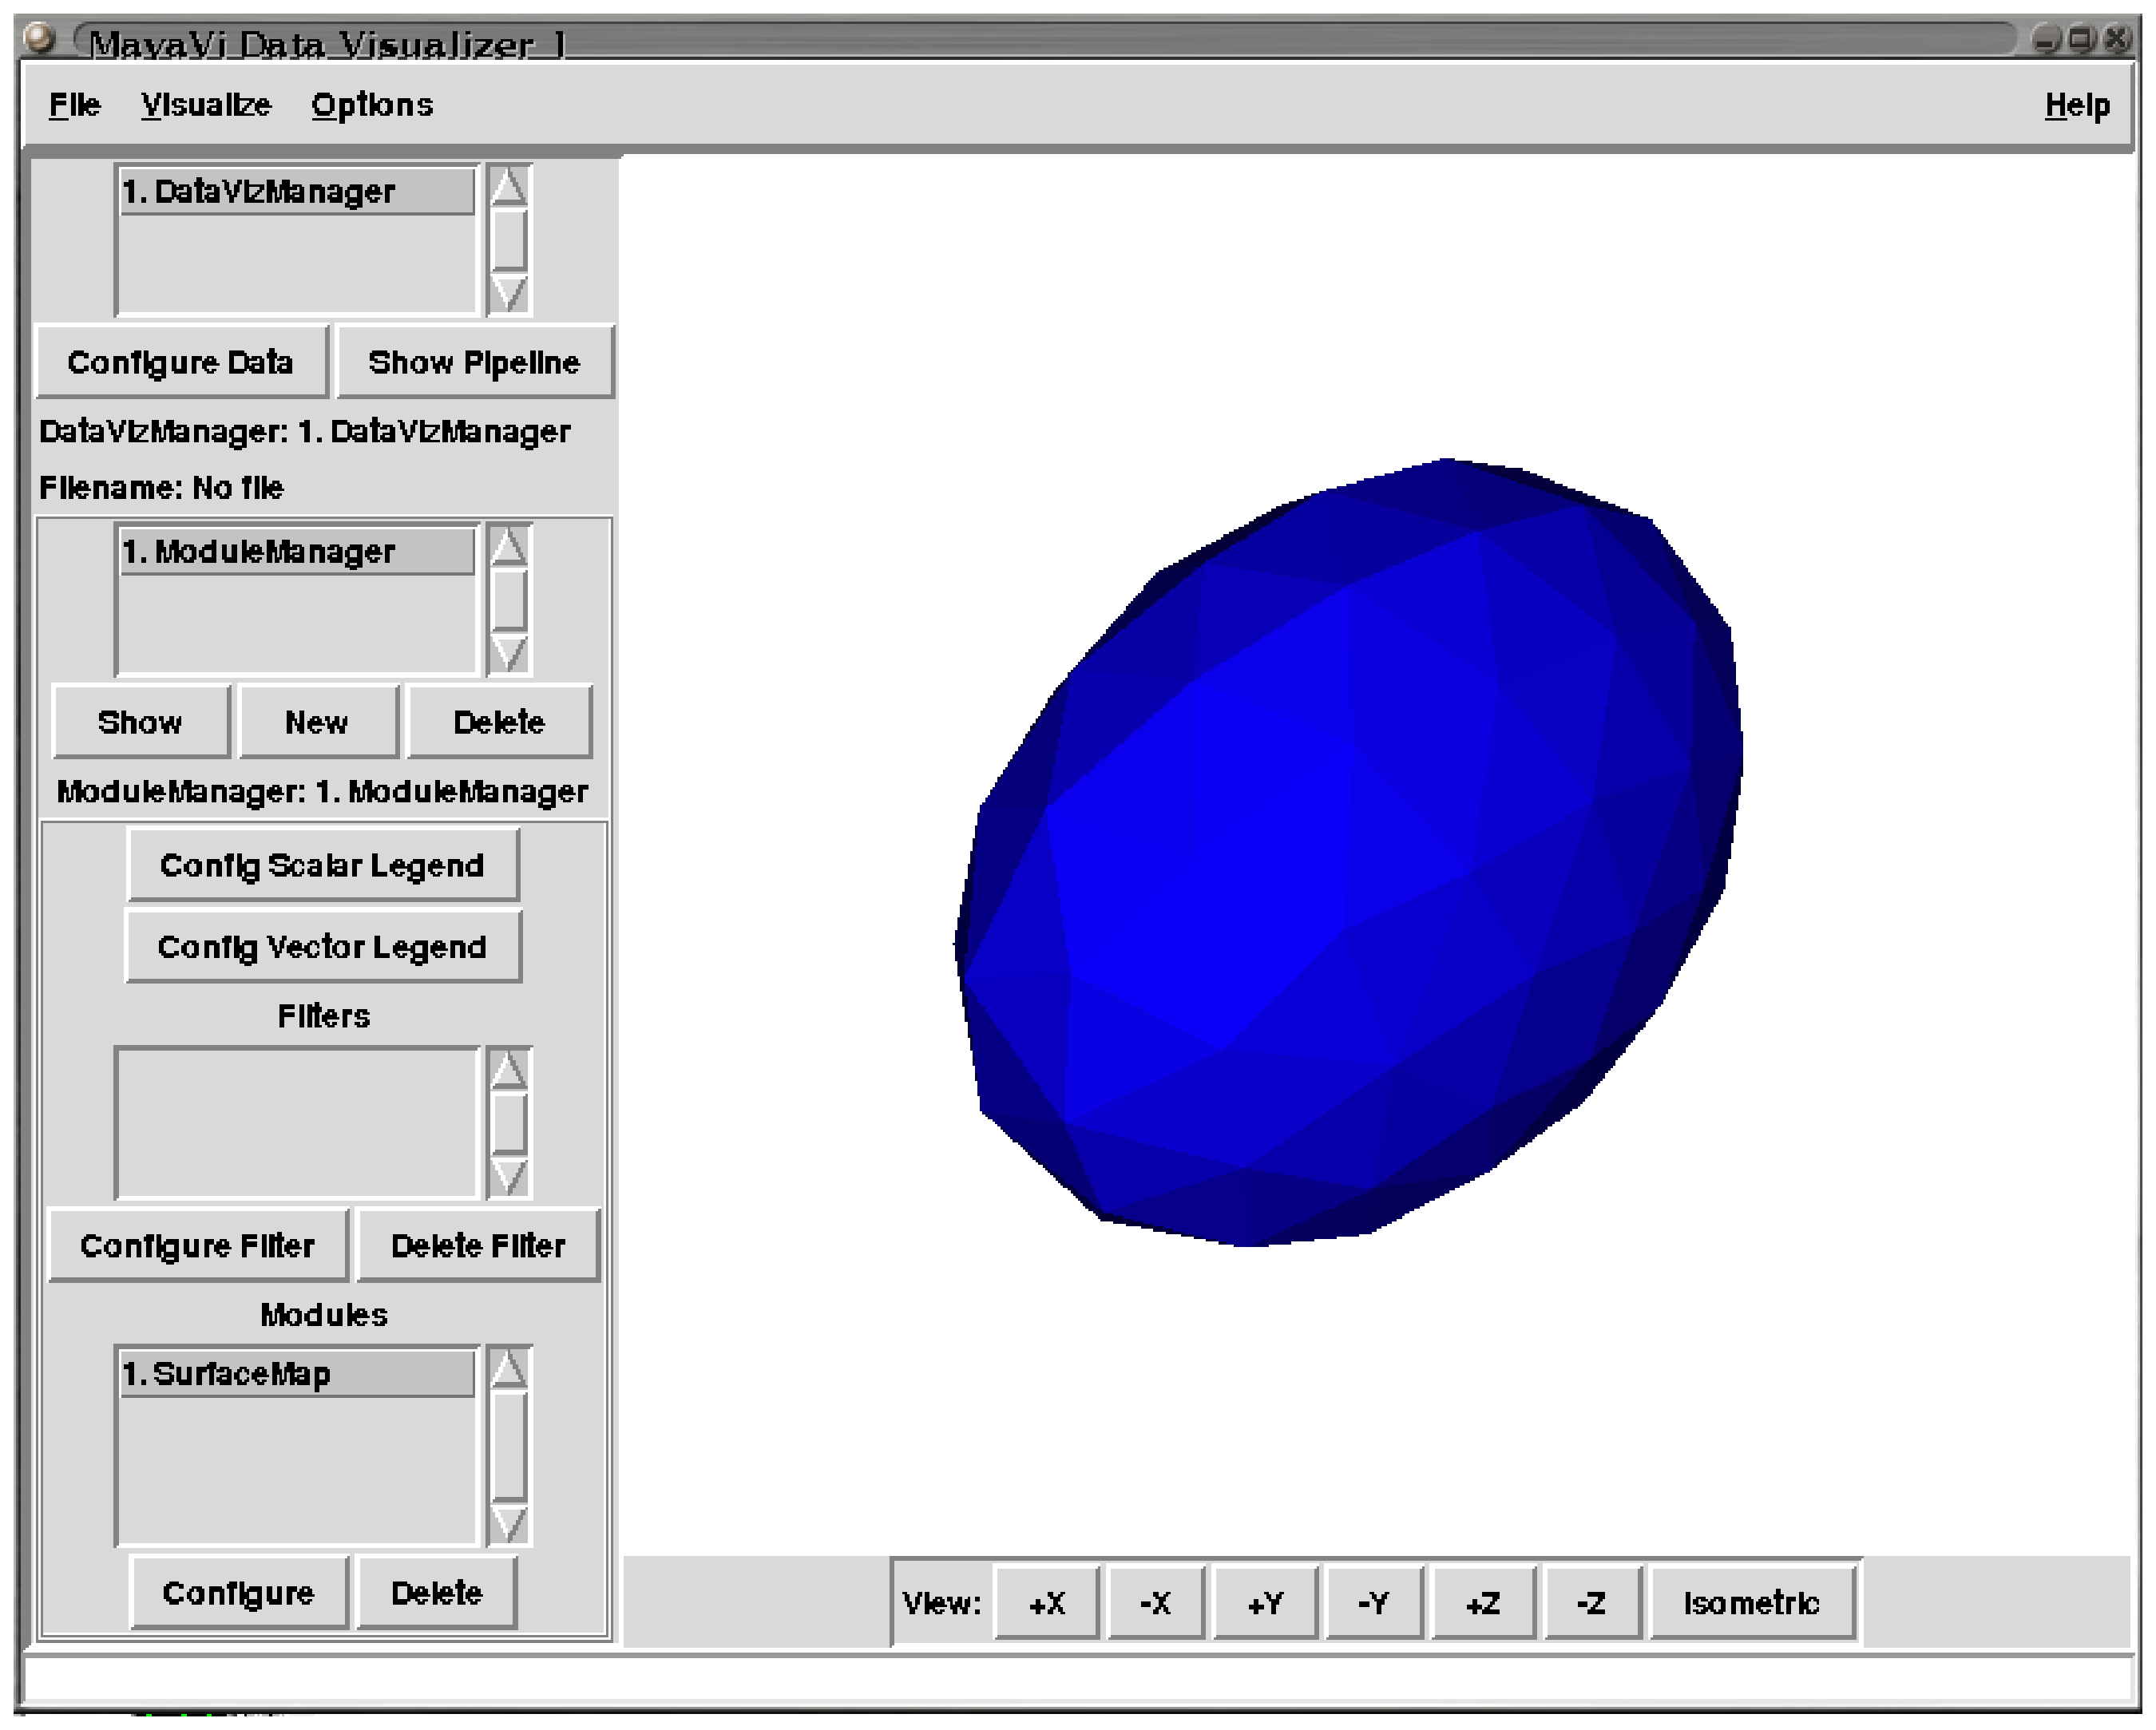
\includegraphics[width=0.3\textwidth]{figures/mayavisnapshot}}
\caption{\label{fig:mayavisnapshot} The MayaVi window (started from \texttt{simple2mayavi.py})}
\end{figure}


%(There is a number of advanced visualisation tools in development.)

\section{Exporting meshes}

\subsection{Exporting meshes from within Python}\label{sec:exporting-meshes}

Once a mesh has been generated (for example such as shown here): 
\lstinputlisting[lastline=7]{../examples/simplemesh.py}

The \texttt{mesh} object provides a number of properties that contain
most of the mesh data. These are:

\begin{itemize}
\item \texttt{mesh.points}: A list of the coordinates of all mesh points.
\item \texttt{mesh.pointsregions}: A list of lists showing in which region a point is located. This can have more than entry if a point is on the boundary between two regions. The outer space has number -1.
\item \texttt{mesh.surfaces}: A list of lists containing indices of points that form the surface elements.
\item \texttt{mesh.surfacesregions}: A list of integers containing the region to which each surface elment belongs.
\item \texttt{mesh.simplices}: A list of lists containing indices of points that form the simplices
\item \texttt{mesh.simplicesregions}: A list of integers containing the region to which each simplex belongs.

\item \texttt{mesh.links}: A list of 2-tuples each containing the coordinates of two mesh points which are connected.

\item \texttt{mesh.dim}: The dimension of the space in which the mesh has been defined.
\end{itemize}

This should provide most of the data that is important for most users. There is a less userfriendly way 
of obtaining some more information about the mesh. This is described in section \ref{sec:exporting-meshes-low-level}.

\subsection{Exporting meshes from within Python, low level command}\label{sec:exporting-meshes-low-level}

Once a mesh has been generated, the \texttt{mesh} object provides a
method to return the metadata as a list of lists to the user. The list
of lists is (by convention) called \texttt{meshinfo}:

\lstinputlisting{../examples/simplemesh.py}

We start \nsimi and execute \texttt{simplemesh.py} as follows:

\begin{lstlisting}
In [1]: run simplemesh.py
\end{lstlisting}
Note that \verb|In [1]: | is the ipython prompt and not part of the command.

Once the execution has finished, we can inspect the \texttt{meshinfo}
object. We find that the \texttt{meshinfo} list has a length of 5.
Each of the 5 entries is a list that provides a keyword (in position
0), a more detailed explanation of the data (in position 1), and
actual data (in position 2). 

Here are some extracts of this interactive session:

\begin{lstlisting}
In [1]: run simplemesh.py
       root:2006-09-15 15:29:04,333   nbase.py  426    INFO run_id is 'simplemesh'
<snip>
 
In [2]: len(meshinfo)
Out[2]: 5

In [3]: meshinfo[0][0]
Out[3]: 'COORDS'

In [4]: meshinfo[0][1]
Out[4]: 'Coordinates of points'

In [5]: meshinfo[0][2][0:5]
Out[5]: 
[[-1.2259282541884986, -0.14647857088992958],
 [0.39556386486232231, -0.71145662309436664],
 [-1.1578161106146379, 0.2826769841571467],
 [1.1583272390040285, -0.28192213952053896],
 [-0.95784703497849266, -0.48188220822162603]]

# For this 2d mesh, point 0 is located at 
# x=-1.2259282541884986 and y -0.14647857088992958 
# ...
In [6]: meshinfo[1][0]
Out[6]: 'LINKS'

In [7]: meshinfo[1][1]
Out[7]: 'Links in the mesh (pairs of point indices)'

In [8]: meshinfo[1][2][0:5]
Out[8]: [(6, 5), (25, 24), (19, 18), (23, 22), (2, 0)]

# These are connections between nodes (i.e. surface elements)

In [9]: meshinfo[2][0]
Out[9]: 'SIMPLICES'

In [10]: meshinfo[2][1]
Out[10]: 'Simplex info (points-coords,((circumcirc center,cc radius),
         (ic center,ic radius),region))'

In [11]: meshinfo[2][2][0:5]
Out[11]: 
[([21, 10, 3],
  ([0.8951112182084433, -0.30657565775478746], 0.26436805700535826),
  ([0.95927847769327945, -0.28831579971465743], 0.12376610605044097),
  1),
 ([23, 17, 22],
  ([0.3813486959002757, 0.17950246466300987], 0.23544275340531229),
  ([0.35011255785332634, 0.21579823153665204], 0.11285166000960006),
  1),
 ([9, 24, 4],
  ([-0.69857851907551072, -0.46117596803433558], 0.2600940439941456),
  ([-0.71080317352675948, -0.45457799374543567], 0.12967604956301398),
  1),
 ([16, 21, 22],
  ([0.59756230001690303, -0.029844435174023323], 0.24555948330679339),
  ([0.679065640872756, -0.026024609120838715], 0.10922419586039551),
  1),
 ([17, 16, 22],
  ([0.46807199985021408, -0.0050280591435365157], 0.26419597795648747),
  ([0.43795013536622696, -0.011585825241475407], 0.13029945475463889),
  1)]

# These are the volume elements (simplices), i.e. the first volume 
# element connects points 21, 10 and 3. Some additional properties 
# of each simplex is provided.

In [12]: meshinfo[3][0]
Out[12]: 'POINT-BODIES'

In [13]: meshinfo[3][1]
Out[13]: 'Which bodies does the corresponding point belong to 
          (body index list)'
In [14]: meshinfo[3][2][0:5]
Out[14]: [[-1, 1], [-1, 1], [-1, 1], [-1, 1], [-1, 1]]

# Each object that we request to be meshed has a body number. The 
# outer space has number -1. Point 0 is just on the surface of body 
# 1 as it is also part of body -1 (the outer space).

In [15]: meshinfo[4][0]
Out[15]: 'SURFACES'

In [16]: meshinfo[4][1]
Out[16]: 'Surface elements info (points-coords,((circumcirc center,cc radius),
         (ic center,ic radius),region))'

In [17]: meshinfo[4][2][0:5]
Out[17]: 
[([6, 5],
  ([1.0915999980528599, 0.31465115148616185], 0.21454721764237583),
  ([1.0915999980528599, 0.31465115148616185], 0.21454721764237583),
  1),
 ([2, 0],
  ([-1.1918721824015681, 0.068099206633608564], 0.21726352347436878),
  ([-1.1918721824015681, 0.068099206633608564], 0.21726352347436878),
  1),
 ([4, 0],
  ([-1.0918876445834957, -0.31418038955577782], 0.21468764521302536),
  ([-1.0918876445834957, -0.31418038955577782], 0.21468764521302536),
  1),
 ([9, 4],
  ([-0.75334144580139872, -0.57786117026132933], 0.2259081608948405),
  ([-0.75334144580139872, -0.57786117026132933], 0.2259081608948405),
  1),
 ([11, 6],
  ([0.75310820256293187, 0.57800212277646423], 0.22576341406349751),
  ([0.75310820256293187, 0.57800212277646423], 0.22576341406349751),
  1)]

# More data on the surface elements is provided (this is usually only 
# of interest if one wants to analyse the quality of these elements).

\end{lstlisting}

\subsection{Exporting meshes by reading the nmesh file}\label{sec:exporting-meshes-nmeshfiles}
The mesh file format is (currently just a text file and) fairly
straight forward. It can be read by any other programming
language/tool and be converted into the desired format.




\appendix

\chapter{Advanced: Call back functions and monitoring}
\label{chap:callbackfunctions}

\section{Providing a call back function (\texttt{callback.py})}

\lstset{basicstyle=\ttfamily}
The mesher can be provided with a call back function that is called
every $n$ iterations in the computation process of the mesh. This can
be used to provide real time visualisation of the meshing process or
to study for example the mesh quality is a function of iterations.

The basic idea is to call the mesher with a call back function \py{f} and a number $n$ in the following fashion:
\begin{lstlisting}
mesh = nmesh.mesh(objects = [...] callback = (f,n))  
\end{lstlisting}

Here is a complete example:
\lstinputlisting{../examples/callback.py}

The call back function (\py{my\_fun} in the above example) is given three arguments:
\begin{itemize}
\item The \py{piece\_nr}. This is an integer labelling the different objects to be meshed. If the bounding box is meshed, it carries the piece number 0.
\item The \py{iteration\_nr}. This is the counter of the iterations within the mesher.
\item The \py{mesh\_info}. This is the same Python list given by the command
  \py{mesh.tolists()} in section \ref{sec:tolists} for the mesh that is currently being computed. 
\end{itemize}

\section{Access to the mesh from Python (\texttt{tolists.py})}
\label{sec:tolists}
The data contained in a mesh object \texttt{mesh} can be extracted to
a python list of lists with the command \py{mesh.tolists()} as shown
in the following program

\lstinputlisting{../examples/tolists.py}
The resulting list contains these information:
\begin{itemize}
  \item[-] COORDS = Coordinates of points;
  \item[-] LINKS = Connections within the mesh (pairs of point indices);
  \item[-] SIMPLICES = Information on the simplices through points
    coordinates, circumcircle centre and radius, inincircle centre and
    radius and region the simplices belong to;
   \item[-] POINT-BODIES = Which bodies does the corresponding point
     belong to (body index list); 
   \item[-] SURFACES = Information on surface elements through points
     coordinates, circumcircle centre and radius, incircle centre and
     radius and region the elements belong to.
\end{itemize}
Section \ref{sec:exporting-meshes} provides some more details.

%##############################################################################





%\chapter{Advanced:Visualising meshes \label{chapter:visual}}
%
%Note that this section has been contributed, and support may be poorer than for the remaining part of the project.
%
%This chapter has been contributed by James Kenny \texttt{(jck103@soton.ac.uk)}.
%
%%\documentclass[10pt,a4paper]{book}
%        
%\usepackage{amssymb}% for numbers/numbers
%\usepackage{lscape}
%
%\usepackage{sectsty}
%\allsectionsfont{\sffamily}
%
%\setlength{\textheight}{24cm}
%\setlength{\textwidth}{15.912cm}
%
%\setlength{\evensidemargin}{0cm}
%\setlength{\oddsidemargin}{0cm}
%
%\setlength{\topmargin}{-0.5cm}
%%\setlength{\parindent}{0cm}
%
%
%\usepackage{listings}
%\usepackage{color}
%\lstdefinestyle{defaultstyle}{}
%\lstset{language=Python}
%\lstset{basicstyle=\ttfamily}
%\lstset{showstringspaces=fales}
%\lstset{keywordstyle=\color{blue}}
%\lstset{frame=single}
%%\lstset{backgroundcolor=\color{white},emph={EMPTY},emphstyle=\color{white}}
%%\definecolor{lightgrey}{cmyk}{0.1,0.1,0.1,0}
%%\lstset{backgroundcolor=\color{lightgrey}}
%
%\renewcommand{\labelitemii}{\ensuremath{\triangleright}}    %  open triangle replaces default dash
%
%\newcommand{\py}[1]{\texttt{\color{blue}#1}}
%
%\newcommand{\nmesh}{nmesh}
%
%
%
%\usepackage{graphicx}
%
%\usepackage[dvips=true,bookmarks=true]{hyperref} 
%
%
%
%
%
%\begin{document}
\chapter{Visualising meshes \label{chapter:visual}}

This chapter aims to provide a concise introduction to the intended use of the {\ttfamily nmesh.visual} library. It is a collection of Python functions for the manipulation of mesh data with an emphasis on visualisation. Some of the functions for mesh manipulation could potentially be useful for other applications however. The library was created with flexibility in mind, many different effects can be achieved through combining the use of several different functions. This manual explains the usage and purpose of each function, a few examples are given of how to use combinations of functions. For most figures, the caption refers to a script which creates a similar visual. These files can be found in the {\ttfamily /examples} folder of {\ttfamily nmesh}. Thereafter, the user is left to decide which combination is required for the process they seek. 

The source code file {\ttfamily visual.py} contains all of the functions for {\ttfamily nmesh.visual}. This file can be used as a module in its own right, from a Python interpreter in the same directory one can import the library in the following way:
\begin{lstlisting}
>>> import visual
\end{lstlisting}
This manual expects the reader to be using {\ttfamily nmesh} in which case the visual library is found as {\ttfamily nmesh.visual}. If the reader is using the tools outside of the {\ttfamily nmesh} module, whenever {\ttfamily nmesh.visual.some\_function()} is seen it should be replaced with {\ttfamily visual.some\_function()}.

{\ttfamily visual.py} can also be used directly from the command line. To see the options available enter the following at a command prompt:
\begin{lstlisting}
>>> python visual.py --help
\end{lstlisting}
From the command line, VTK files and {\em pickle} files can be used (see section \ref{sec:pickle}). 





\section{Basic structure of a mesh \label{sec:meshinf}}

{\ttfamily nmesh} meshes are created in the language OCaml and cannot be easily accessed from Python, which is the language used in {\ttfamily nmesh.visual}. One of the methods of a mesh is {\ttfamily mesh.tolists()}, this converts the useful information about a mesh from OCaml, to a list of Python lists. As a convention, the output of {\ttfamily mesh.tolists()} will be referred to as {\ttfamily mesh\_info} from here on.

\begin{figure}
\begin{center}
\includegraphics[width=\textwidth]{visualfigures/meshinfo1}
\caption{{\em The output of} {\ttfamily mesh.tolists()}. \label{fig:meshinfo1}}
\end{center}
\end{figure}

The basic structure of this list is shown in figure \ref{fig:meshinfo1}. There are five lists within {\ttfamily mesh\_info}, the first element of each list is a string containing the title of the list. These titles must be as shown in the diagram, because this is how {\ttfamily nmesh.visual} finds the data it needs. However, it means that these lists do not have to appear in any particular order. The minimum number of lists is two, because the data associated with {\ttfamily ``COORDS''} and {\ttfamily ``SIMPLICES''} is required to define a mesh.

The second element of each list is a description of the data within that list, for example: {\ttfamily mesh\_info[0][1] = 'Coordinates of points'}. Finally, the third element of each list is itself another list (or tuple), containing the data. 

The five data headings in {\ttfamily mesh\_info} are {\ttfamily ``COORDS''}, {\ttfamily ``LINKS''}, {\ttfamily ``SIMPLICES''}, {\ttfamily ``POINT-BODIES''} and {\ttfamily ``SURFACES''}.  'Coords' contains a list of the coordinates for points (nodes) on the mesh, 'links' contains a list of pairs of integers. Each integer is the list index for a point in 'coords', these pairs of indices describe the connections in a mesh. The 'simplices' header contains a list of simplices, the first part of each simplex entry has a list of three or four indices for the 'coords' list. Three indices define a triangle and four define a tetrahedron. The second and third entries in a simplex describe the position of its circumcentre and incentre, and its circumradius and inradius. The final entry in a simplex is another integer, this is the part index and explains which part of the mesh this simplex belongs to. The data following the 'point-bodies' header is a list of tuples, some may be single element tuples. These tuples describe which part of the mesh a point in the 'coords' list belongs to. A tuple {\ttfamily (-1,1)} would mean that the point in question is on the border between part -1 (the void outside the mesh) and part 1. These tuples occur in the same order as the points in the list 'coords', so the third tuple in this list describes which part(s) the third point in 'coords' belongs to. Finally, the data associated with the 'surfaces' heading is essentially more simplex data. The difference is that for a 3D mesh, simplices will be tetrahedra and surfaces will be triangles and for 2D meshes surfaces will be lines. At the time of writing, the data available in 'surfaces' was limited.

To find out the exact format of data in the third element of each of these lists, the reader should load a {\ttfamily mesh\_info} in the Python interpreter and manually view one of the elements. For example, to view the format of simplices data, type the following:
\begin{lstlisting}
>>> mesh_info[simplices][2][0]
\end{lstlisting}
This will print the first element of the data list, under the {\ttfamily ``SIMPLICES''} heading.



\section{Saving and loading mesh data \label{sec:pickle}}
A mesh object can be saved by using the following method: {\ttfamily mesh.save(<filename>)}, this saves the mesh in a form that OCaml can read, but Python cannot. It is useful to be able to save {\ttfamily mesh\_info} lists, this can be done using the function 
{\ttfamily nmesh.visual.pickle(<filename.dat>)}. In this manner the information about the mesh is saved in such a way that OCaml is not required. So this data could be sent to a third party, along with the file {\ttfamily visual.py} which contains the source code for {\ttfamily nmesh.visual}. Providing that Python is available on their system, it will be possible for them to analyse the mesh. The accompanying function 
{\ttfamily nmesh.visual.unpickle()} should be used to retrieve {\ttfamily mesh\_info} from a pickled file.




\section{Manipulating mesh data}
All of the functions described in this section can be used to take information from {\ttfamily mesh\_info} and deposit some, or all of it, in a new container (say {\ttfamily mesh\_info2}) in a slightly different form. The output, {\ttfamily mesh\_info2}, has the same format as the input and can be used in the same way. All functions in this section will remove the data {\ttfamily ``LINKS''}. 

\subsection{{\ttfamily separate\_parts()}}
This function separates the elements of a mesh according to which {\em part} they belong to. If for example a mesh contains a cone and a cube, these will generally be considered as distinct parts. Each simplex in a mesh has an index describing which part it belongs to. If in this example all the simplices of the cone have indices of $1$ and the simplices of the cube have indices of $2$, the following command would create two {\ttfamily mesh\_info} style lists; the first containing the mesh information for the cone and the second for the cube:

\begin{lstlisting}[basicstyle=\small\ttfamily]
>>> [cn, cb] = nmesh.visual.separate_parts(mesh_info, listOfParts=[[1],[2]])
\end{lstlisting}



From this the reader can see that the output of {\ttfamily separate\_parts()} is a list, each element of which is the {\ttfamily mesh\_info} for the part (or group of parts) requested. These will occur in the same order in the output as they were given in the argument {\ttfamily listOfParts}. This input argument is mandatory, if it is not given the function will not run. {\ttfamily listOfParts} can either be an integer (when only one part it required), or a list of lists. The output is always a list. The following two commands achieve the same thing:
\begin{lstlisting}[basicstyle=\small\ttfamily]
>>> [part] = nmesh.visual.separate_parts(mesh_info, listOfParts=1)
>>> [part] = nmesh.visual.separate_parts(mesh_info, listOfParts=[[1]])
\end{lstlisting}
However, the following command would raise an error:
\begin{lstlisting}[basicstyle=\small\ttfamily]
>>> [part] = nmesh.visual.separate_parts(mesh_info, listOfParts=[1])
\end{lstlisting}
This is because {\ttfamily listOfParts} is expected to be a list, if it is an integer, it is wrapped in a nested list. If however a list is provided, but it is not a list of lists, the function will try to iterate over a non-existent sequence.


The reader is invited to examine the following code and ascertain what it does, the solution follows.
\begin{lstlisting}[basicstyle=\small\ttfamily]
>>> info = nmesh.visual.separate_parts(mesh_info, listOfParts=[[1,2,3],[8,9]])
>>> group1 = info[0]
>>> group2 = info[1]
\end{lstlisting}
The answer is, that the mesh associated with {\ttfamily mesh\_info} has been split into two pieces. The first contains parts 1, 2 and 3; the second contains parts 8 and 9. The output was assigned to a single variable, {\ttfamily info}, so this is in fact a list. Two new variables have been assigned, {\ttfamily group1} takes the {\ttfamily mesh\_info} for parts 1, 2 and 3. {\ttfamily group2} takes the {\ttfamily mesh\_info} for parts 8 and 9. It is worth noting here that any parts in the mesh which are not included in the argument {\ttfamily listOfParts} will be discarded. So in the above example, if there were nine parts, those with indices 4, 5, 6 and 7 have been ignored. Finally, repetition is allowed:
\begin{lstlisting}[basicstyle=\small\ttfamily]
>>> [a, b] = nmesh.visual.separate_parts(mesh_info, listOfParts=[[1],[1]])
>>> [c, d] = nmesh.visual.separate_parts(mesh_info, listOfParts=[[1],[1,2]])
\end{lstlisting}
Whilst this is inefficient, items {\ttfamily a}, {\ttfamily b} and {\ttfamily c} will be the same, containing information for part 1. {\ttfamily d} will have the information for parts 1 and 2 in a single dataset.




\subsection{{\ttfamily surface\_only()}}
This function can be used to display only the surface elements of a mesh. In some ways it is more useful to think of this as the {\em outline} of a mesh. For a three-dimensional mesh of tetrahedra this will result in a surface made up of triangles. For a two-dimensional mesh of triangles this function will return a mesh of lines, forming the outline of the 2D shape that has been meshed. This is illustrated, for the 2D case, in figure \ref{fig:surfaceonly2d}.

\begin{figure}
\begin{center}
\includegraphics[width=0.8\textwidth]{visualfigures/surfaceonly2d}
\caption{{\em A 2D mesh, before and after use of }{\ttfamily surface\_only() (surface\_elements\_bug.py)}. \label{fig:surfaceonly2d}}
\end{center}
\end{figure}

The user can optionally choose to view the surface of only certain parts. In this case the process is similar to {\ttfamily separate\_parts()} in that the return argument is a list of {\ttfamily mesh\_info} type lists. The output of this function is always in a similar format to {\ttfamily mesh\_info}, but contains only the simplices and points on the surface of the mesh; all information about the mesh interior is removed. Examine the following:

\begin{lstlisting}[basicstyle=\small\ttfamily]
>>> s1 = nmesh.visual.surface_only(mesh_info)
>>> s2 = nmesh.visual.surface_only(mesh_info, listOfSurfaces=2)
[s3, s4] = nmesh.visual.surface_only(mesh_info, listOfSurfaces=[[3],[4,5]])
\end{lstlisting}
{\ttfamily s1} will contain the information for the surface of each part in {\ttfamily mesh\_info}. {\ttfamily s2} will contain the information for the surface of part 2 only. {\ttfamily s3} will contain information on the surface of part 3 only and {\ttfamily s4} will contain the data for the surfaces of parts 4 and 5 in a single dataset.

Again, the reader should note that the optional argument {\ttfamily listOfSurfaces} must either be an integer or a list of lists. The surface elements of any mesh are included in the original output of {\ttfamily mesh.tolists()}, so there is very little computational demand in the function {\ttfamily surface\_only()} because it just reads this data from the {\ttfamily ``SURFACES''} element of {\ttfamily mesh\_info} to the {\ttfamily ``SIMPLICES''} element. 




\subsection{{\ttfamily outer\_skin()}}
This function does something slightly different to {\ttfamily surface\_only()}. It does not use the {\ttfamily ``SURFACES''} data from {\ttfamily mesh\_info}, instead, it works out for itself which simplices are near the surface and returns a {\ttfamily mesh\_info} style list of these. In general any simplex containing one or more of the points on the surface of the mesh, will be included in the output. The user can however specify their own condition using the optional input argument {\ttfamily condition}. The function can be used for 2D and 3D meshes, but not for ones where only the surface elements are present (ie: not on meshes which have been processed by {\ttfamily surface\_only()}.

The {\ttfamily condition} argument determines how many points must be in a simplex for it to be included in the output. Read the following lines of code and attempt to figure out their meaning.
\begin{lstlisting}[basicstyle=\small\ttfamily]
>>> skin1 = nmesh.visual.outer_skin(mesh_info)
>>> skin2 = nmesh.visual.outer_skin(mesh_info, condition='>= 1')
>>> skin3 = nmesh.visual.outer_skin(mesh_info, condition='== 2')
>>> skin4 = nmesh.visual.outer_skin(mesh_info, condition='> 2')
\end{lstlisting}

{\ttfamily skin1} will be identical to {\ttfamily skin2} because the default value of {\ttfamily condition} is {\ttfamily '>= 1'}. {\ttfamily skin3} will contain a set of simplices all of whom contain exactly points on the surface of the mesh. {\ttfamily skin4} will have a set of simplices each with more than two surface points. For a 2D mesh this would be an unwise choice, because there may very well be no simplices with three surface points. It is likely in 2D that corner elements will satisfy this however. Similarly, choosing simplices with four surface points for a 3D mesh would be unwise. Whilst these simplices may exist, they are generally a sign of a poor quality mesh. Figure \ref{fig:skinmesh2d} illustrates the outputs of the above lines of code. 

\begin{figure}
\begin{center}
\includegraphics[width=\textwidth]{visualfigures/skinmesh2d}
\caption{{\em From left to right,} {\ttfamily skin1}, {\ttfamily skin3} {\em and} {\ttfamily skin4}. \label{fig:skinmesh2d}}
\end{center}
\end{figure}



\subsection{{\ttfamily order\_mesh()}}
{\ttfamily nmesh.visual} uses a vtkUnstructuredGrid to represent mesh data. Although as the name suggests, this data structure does not impose a strict ordering system, all elements (simplices and points) have an index. The filter {\em ExtractUnstructuredGrid} can be used to view a subset of a vtkUnstructuredGrid by only displaying cells (or points) within a specified range. {\ttfamily order\_mesh()} rearranges a {\ttfamily mesh\_info} such that simplex indices increase along an axis. In this way the filter explained can be used to remove simplices of a mesh in a controllable fashion, so the interior of a 3D mesh can be viewed. Alternatively the user may provide a dataset, with one entry for each simplex, the mesh will then be sorted by this data. 

{\ttfamily order\_mesh()} expects a {\ttfamily mesh\_info} style list, if nothing else is provided, the mesh given will be sorted along the first axis (x-axis) and returned. The user can specify the axis along which the mesh is sorted using the optional argument {\ttfamily axis}. This must be either 0, 1 or 2; corresponding to the x, y and z axes respectively. Alternatively the user may provide a dataset for the mesh to be sorted by, this is done by assigning the optional argument {\ttfamily data}. For example to sort a mesh by the list {\ttfamily quality} the function call would be as follows:
\begin{lstlisting}[basicstyle=\small\ttfamily]
>>> sorted_mesh = nmesh.visual.order_mesh(mesh_info, data=quality)
\end{lstlisting}

As an example, an ellipsoid was meshed and then ordered using the ratio:
\[
3 \times \frac{\mathrm{inradius}}{\mathrm{circumradius}}.
\]
This is a measure of the regularity of a tetrahedron. Regular tetrahedra will have a value of one and the worst tetrahedra will have values approaching zero. Figure \ref{fig:best200} shows the 200 most regular tetrahedra and figure \ref{fig:worst200} shows the 200 least regular tetrahedra. 


\begin{figure}
\begin{center}
\includegraphics[width=0.85\textwidth]{visualfigures/best200}
\caption{{\em The best 200 simplices in a mesh. }(visual\_view\_by\_quality.py) \label{fig:best200}}
\end{center}
\end{figure}


\begin{figure}
\begin{center}
\includegraphics[width=0.85\textwidth]{visualfigures/worst200}
\caption{{\em The worst 200 simplices in a mesh.} \label{fig:worst200}}
\end{center}
\end{figure}


Figure \ref{fig:sweep} shows the same mesh, ordered along the y-axis. The filter ExtractUnstructuredGrid was used to remove a different number of simplices in each sub-image. The call to {\ttfamily order\_mesh()} which created this mesh is shown below.
\begin{lstlisting}[basicstyle=\small\ttfamily]
>>> ordered_mesh = nmesh.visual.order_mesh(mesh_info, axis=1)
\end{lstlisting}

Once a mesh has been ordered, the {\ttfamily mesh\_info} can be used in the same way as the original output of {\ttfamily mesh.tolists()}. Once it has been converted to VTK data and visualised in MayaVi, the filter ExtractUnstructuredGrid must be applied to remove cells selectively. For information on using MayaVi please see the guide produced in section \ref{sec:mayaviguide}. Figure \ref{fig:sweep} shows the effect of changing {\ttfamily CellMaximum} alone. Figure \ref{fig:sweep2} shows how, by varying {\ttfamily CellMaximum} and {\ttfamily CellMinimum} so that a narrow range of simplices is shown, the effect of viewing a layer of simplices can be achieved.


\newpage
\begin{landscape}
\begin{figure}
\begin{center}
\includegraphics[width=9in]{visualfigures/sweep}
\caption{{\em The filter ExtractUnstructuredGrid can be used to cut away parts of a mesh.} (visual\_sweep.py) \label{fig:sweep}}
\end{center}
\end{figure}
\end{landscape}

\newpage
\begin{landscape}
\begin{figure}
\begin{center}
\includegraphics[width=9in]{visualfigures/layers2}
\caption{{\em The filter ExtractUnstructuredGrid can be used to view layers of tetrahedra.} \label{fig:sweep2}}
\end{center}
\end{figure}
\end{landscape}




\subsection{{\ttfamily skin\_mesh()}}
This function uses a similar process to {\ttfamily outer\_skin()} but does so recursively. Whereas {\ttfamily outer\_skin()} reduces a {\ttfamily mesh\_info} to contain information about certain simplices near the surface, {\ttfamily skin\_mesh()} finds those simplices, then the next layer of simplices touching those, etc. The easiest way to describe this is to say that it orders the indices in a mesh such that the filter ExtractUnstructuredGrid can be used to peel back layers of simplices, much like peeling skins from an onion. This function is computationally intensive, this has been tolerated because it is unlikely to be used frequently. 

It is important with this function that the user understand a little more detail about how it works. In a similar way to {\ttfamily outer\_skin()} it finds all the points on the surface of a mesh, then finds the simplices which contain a certain number of those points. The number of points which must be in a simplex can be set by the user in the same way it is for {\ttfamily outer\_skin()}, again the default is {\ttfamily '>= 1'}. Once these simplices are found, all the points within those simplices, which are not points on the surface are put in a list. The function then repeats, searching through this new list of points, simplices which include these points but have not already been indexed form a new layer. Again, a list is made, of the points within these simplices which have not yet been considered. Then the simplices containing those points form the next layer, and so on. This continues until all the points in the mesh have been considered. 

For convenience, the function also returns a list of tuples, each tuple giving the values which should be used for {\ttfamily CellMaximum} and {\ttfamily CellMinimum} in the filter ExtractUnstructuredGrid. An example can be seen in figure \ref{fig:onion}, there the condition used was the default. The reader should consider the effect of changing the condition. For example, changing the condition to be {\ttfamily '>= 3'}, will include only those simplices with three or more surface points in the outer layer. Then the simplices with three or more of the remaining points in the next layer, etc. This will mean there are more layers and will significantly increase the runtime of the function. The user should be aware that the {\ttfamily mesh\_info} given as input argument to this function will be partially destroyed, this is necessary to increase the efficiency of the routine. The user should employ {\ttfamily copy.deepcopy()} to replicate {\ttfamily mesh\_info} before it is passed to {\ttfamily skin\_mesh()}, if the  user wishes to retain the original mesh data.


The output from this function is the same as any other {\ttfamily mesh\_info} and can be passed to other functions, just as the output of {\ttfamily mesh.tolists()}. The command used to order the mesh for figure \ref{fig:onion} is shown below.
\begin{lstlisting}[basicstyle=\small\ttfamily]
>>> layers, intervals = nmesh.visual.skin_mesh(mesh_info, condition='>=1')
\end{lstlisting}



\newpage
\begin{landscape}
\begin{figure}
\begin{center}
\includegraphics[width=9in]{visualfigures/onion}
\caption{{\em The end effect of using }{\ttfamily skin\_mesh()}{\em and ExtractUnstructuredGrid. }(visual\_skinning.py) \label{fig:onion}}
\end{center}
\end{figure}
\end{landscape}



\section{Processing VTK data}
The functions described in this section are all related to creating and handling VTK datasets. {\ttfamily nmesh.visual} exclusively uses vtkUnstructuredGrid datasets, these should be appropriate for any work with meshes from {\ttfamily nmesh}. 

\subsection{{\ttfamily mesh2vtk()}}
This function takes a {\ttfamily mesh\_info}, either in its original form or after manipulation by the functions from the previous section. It creates a vtkUnstructuredGrid dataset from it, automatically deciding when to use triangles or tetrahedra. If the user wishes, additional information about the mesh can be provided. This does not increase runtime because these data are generated in any case. This extra data is returned by changing the input argument {\ttfamily VTKonly} to be False. The following lines show the two possible calls to this function:
\begin{lstlisting}[basicstyle=\small\ttfamily]
>>> vtkData = nmesh.visual.mesh2vtk(mesh_info)
>>> data = nmesh.visual.mesh2vtk(mesh_info, VTKonly=False)
\end{lstlisting}
The first line produces a VTK dataset called {\ttfamily vtkData}, this can be visualised in MayaVi or have additional data appended to it by {\ttfamily append2vtk()}. The second line produces a list called {\ttfamily data}. The first element of this list is the same VTK dataset, the second element of the list is a list of the points in the mesh. These points will be in three dimensions even if the input mesh was only in two dimensions. The third element of {\ttfamily data} will be a list of triangles or tetrahedra. Each shape is simply a list of three or four indices of points in the list contained in the second element of {\ttfamily data}. The fourth element is a list of the indices describing which part each simplex belongs to. The fifth element of {\ttfamily data} is a list of the incircle radii for the simplices and the sixth element is a list of the circumcircle radii.

There are many possible applications for the additional data output by {\ttfamily mesh2vtk()}. The list of simplex indices can be appended to the VTK dataset as cell data, this way all the cells of a part will share the same value. This can be useful for displaying different parts in different colours. Also, the lists of inradii and circumradii can be sent to {\ttfamily findRatios()} and a useful quality metric is returned. This quality metric can be appended to the VTK data as cell data and each simplex of the mesh can be coloured according to its quality; this is exceptionally useful for the visual analysis of mesh quality. Alternatively, this quality data could be analysed statistically, perhaps to find the mean quality or to plot a histogram. 



\subsection{{\ttfamily append2vtk()}}
A vtkUnstructuredGrid, as produced by {\ttfamily mesh2vtk()} can have a variety of additional data added to it. This data can either be associated with the points in the grid ({\em point data}), or with the cells ({\em cell data}). {\ttfamily append2vtk()} simplifies the process of adding either type of data to a mesh. As described in the last paragraph of the previous section, the part indices for each simplex could be appended:
\begin{lstlisting}[basicstyle=\small\ttfamily]
>>> vtkData2 = nmesh.visual.append2vtk(vtkData, indices, "Part indices")
\end{lstlisting}
The VTK dataset is given first, then the data to be appended to it and finally a title for the data set. The resulting VTK data has been visualised in figure \ref{fig:partindices}, the reader can see that each part has a different colour. This is because a colour scale, dependent upon the part index, has been applied. Figure \ref{fig:in2circdata} shows a different scalar data set applied as cell data to a mesh. In this case the mesh is of a frustum, the cells have been coloured according to their regularity. More regular cells are blue, highly irregular cells are red.


\begin{figure}
\begin{center}
\includegraphics[width=0.85\textwidth]{visualfigures/partindices}
\caption{{\em A mesh with simplices coloured by which part they belong to. }(visual\_separate\_parts.py) \label{fig:partindices}}
\end{center}
\end{figure}


\begin{figure}
\begin{center}
\includegraphics[width=0.85\textwidth]{visualfigures/in2circdata}
\caption{{\em A mesh where simplices have been coloured according to their regularity.} (visual\_in2circ2d.py) \label{fig:in2circdata}}
\end{center}
\end{figure}


By default data sets are appended as cell data, but by changing the optional argument {\ttfamily sites} to be {\ttfamily 'point'}, data can be appended to points instead. If the list of data to be appended does not have an entry for each site, an error will arise. To clarify, a mesh with say 500 simplices, must be given a list of cell data with 500 values. An example of a mesh with point data appended to it is shown in figure \ref{fig:pointdata}. In this case the data is vectors showing the direction of a magnetic exchange field, the mesh is of a bar viewed along its axis. {\ttfamily append2vtk()} allows 3D vector, or scalar data for point data. Cell data can only be scalar data. This limitation is imposed by {\ttfamily append2vtk()} not be VTK's data structures.

\begin{figure}
\begin{center}
\includegraphics[width=0.5\textwidth]{visualfigures/pointdata}
\caption{{\em A mesh with vector point data appended. }(example\_for\_tf.py) \label{fig:pointdata}}
\end{center}
\end{figure}



\subsection{{\ttfamily findRatios()}}
This function accepts two lists and returns a single list of the same length. The i'th element of the returned list is found by dividing the i'th element of the first input list, by the i'th element of the second input list. Optionally the argument {\ttfamily factor} can be set, this way each element of the returned list will have been multiplied by the value of {\ttfamily factor}. This function is useful because many of the quality metrics for unstructured meshes are found by dividing one property by another. For example, a good measure of the regularity of a triangle or tetrahedron is:
\[
\frac{\mathrm{inradius}}{\mathrm{circumradius}}.
\]
When multiplied by a factor of 2 for triangles or a factor of 3 for tetrahedra, this value will be unity for a regular shape and approach zero for distorted shapes. This metric was applied to the mesh in figure \ref{fig:in2circdata}. It was calculated with the following entry and then applied to the VTK data by use of {\ttfamily append2vtk()}.
\begin{lstlisting}[basicstyle=\small\ttfamily]
>>> in2circ = nmesh.visual.findRatios(icradii, ccradii, factor=3)
\end{lstlisting}
The returned list is one-dimensional.


\subsection{{\ttfamily findAngles()}}
This function finds all of the internal angles of a triangular mesh. Typically this data is used to plot a histogram, a good mesh will predominantly have angles of $60^{o}$. To create a list of all the internal angles of a mesh the following command should be used.
\begin{lstlisting}[basicstyle=\small\ttfamily]
>>> angles = nmesh.visual.findAngles(mesh_info)
\end{lstlisting}
The returned list is a list of three element lists. Each three element list contains the internal angles of a triangle. It would therefore be possible to reduce the list to contain the largest, or the smallest, angle for each triangle and append this to a mesh as cell data. To append the data using {\ttfamily append2vtk()} the user would first have to make the list one-dimensional, this can be done by using the {\ttfamily ravel} function from the {\ttfamily Numeric} libraries:
\begin{lstlisting}[basicstyle=\small\ttfamily]
>>> import Numeric
>>> linear-list = Numeric.ravel(list)
\end{lstlisting}




\subsection{{\ttfamily save\_vtk()}}
This function simply allows the user to save a VTK dataset to a file in the following manner.
\begin{lstlisting}[basicstyle=\small\ttfamily]
>>> nmesh.visual.save_vtk(vtkData, "mesh.vtk")
\end{lstlisting}
The first argument is the VTK dataset to be saved, the second is the file to save it to. The reader is advised to stick to the convention of naming these files with the extension {\ttfamily .vtk}. These files can be viewed by anyone with a VTK visualiser, such as MayaVi.

Saving your VTK data is not only useful to view results at a later stage or on another machine; it is also the only way of making data available to MayaVi on systems where the library {\ttfamily vtkpython} is not present.





\section{Visualising VTK data with MayaVi}
This section describes the use of {\ttfamily nmesh.visual} visualisation functions. A guide to using MayaVi is a separate issue and has been provided in section \ref{sec:mayaviguide}.

\subsection{{\ttfamily mesh2mayavi()}}
This function accepts either a VTK dataset as it's input, or the filename for a VTK file as a string. If the VTK data is not provided as a file, {\ttfamily vtkpython} must be present on the system. There is also a minor memory leak associated with the function in this case. Therefore, in general, the reader is advised to save data to a file first. 

There are a few options available to the user with this function. The handle on an existing MayaVi window can be provided by assigning the optional argument {\ttfamily myv}. This will cause the visualisation to appear in an existing window, rather than opening a new one. The function returns the handle on the MayaVi window it uses, so if one was provided it is returned; if not, a handle on the window which was created by {\ttfamily mesh2mayavi()} will be returned.

The argument {\ttfamily module} can be given a string which is the name of the module to be loaded in MayaVi. By default the SurfaceMap module is used, but other suitable options could be Outline, Axes or Glyph. Finally, if the VTK dataset has cell data appended to it, MayaVi will automatically apply colour scaling to the mesh. This uses a Look-Up-Table (LUT) to assign a different colour to different values of the cell data. The user can specify the range of this colour scale by assigning a two element tuple to the argument {\ttfamily lut\_range}. For example, with the ratio used in figure \ref{fig:in2circdata} the range {\ttfamily lut\_range=(0,1)} was specified.

Please read the following lines and try to decide what they will do. The variable {\ttfamily v} is a handle on a MayaVi window, ie: {\ttfamily v = mayavi.mayavi()}.
\begin{lstlisting}[basicstyle=\small\ttfamily]
>>> v1 = nmesh.visual.mesh2mayavi(vtkData, myv=v)
>>> v2 = nmesh.visual.mesh2mayavi("mesh.vtk", lut_range=(0,10))
\end{lstlisting}
The first line of code visualises a VTK dataset from memory, using the existing MayaVi window handled by {\ttfamily v}. The second line creates a new MayaVi window and displays the data from file {\ttfamily mesh.vtk} in it. The colour scale used in the second example is forced to span data in the range 0 to 10.


\subsection{{\ttfamily rotate()}}
This function simply alters the position from which a mesh is viewed in a MayaVi window. The inputs are {\ttfamily myv} which is the handle on the MayaVi window in question, and a value in degrees for the roll, pitch or yaw required. If none of the angles are specified the view is not changed. All angles are optional, so the view can be rolled but not pitched, etc. Any angle can be given for roll or yaw, the angle given for pitch will yield confusing results if less than $-85^{o}$ or greater than $+85^{o}$. The function does not return anything.

Please consider the following lines, where v is the handle on a MayaVi window.
\begin{lstlisting}[basicstyle=\small\ttfamily]
>>> rotate(v)
>>> rotate(v, roll=20, yaw=-10)
>>> rotate(roll=5, pitch=5, yaw=5)
\end{lstlisting}
The first line does nothing, because no rotations are requested. The second line rotates the view by $+20^{o}$ and $-10^{o}$. The third line will raise an error, because the function has not been told which MayaVi window to apply these changes to.

\subsection{{\ttfamily export\_visualisation()}}
To save an image from a MayaVi window this function should be used. It requires the handle on a MayaVi window and a filename as a string, for it's inputs. The format of the saved picture will be {\ttfamily .png} or {\ttfamily .eps} depending upon the filename given. In actuality, if a {\ttfamily .eps} is requested, a {\ttfamily .eps.gz} will be saved. This should be uncompressed before used in \LaTeX but can be left untouched for viewing in GhostView. It is important to note that this function works by capturing the image on the screen, so if another window is over the top of the MayaVi window, this will be included in the saved image as well. No simple method for off screen rendering exists.

Examine the following:
\begin{lstlisting}[basicstyle=\small\ttfamily]
>>> nmesh.visual.export_visualisation(v, "mesh.png")
>>> nmesh.visual.export_visualisation(v, "mesh.eps")
\end{lstlisting}
The first line saves a {\ttfamily .png} file and the second saves a {\ttfamily .eps.gz} file. Note that this function can only save {\ttfamily .png} files on Microsoft Windows systems. The facility to save {\ttfamily .eps} works only on Linux and UNIX machines.



\section{High-level convenience functions}
\subsection{{\ttfamily basic\_solid()}}
This function uses a sequence of the functions mentioned so far to visualise a mesh as a solid, green in colour. The index describing which part each simplex belongs to is appended, but not used to colour the mesh. The function requires a {\ttfamily mesh\_info} as input. Optionally the user can opt to view only a selection of the parts in the mesh by specifying {\ttfamily part} in the same way as {\ttfamily listOfParts} for {\ttfamily separate\_parts()}. Similarly, the mesh can be ordered using {\ttfamily order\_mesh()} by giving the optional input argument {\ttfamily order} an integer value between zero and two. Ordering can only be chosen when the argument {\ttfamily part} is not given, or is an integer. Finally, this function will draw in an existing MayaVi window if given the handle as argument {\ttfamily myv}.

Examine the following code.
\begin{lstlisting}[basicstyle=\small\ttfamily]
>>> v1 = nmesh.visual.basic_solid(mesh_info)
>>> nmesh.visual.basic_solid(mesh_info, part=1)
>>> v2 = nmesh.visual.basic_solid(mesh_info, order=2, myv=v)
>>> v3 = nmesh.visual.basic_solid(mesh_info, part=[[1,2],[2,3]], order=1)
\end{lstlisting}
Line one simply generates an image of the mesh described by {\ttfamily mesh\_info}. Line two visualises only part 1 of the mesh in {\ttfamily mesh\_info}, also in this situation the returned MayaVi window handle has not been captured. The third line displays the mesh in the existing MayaVi window with the handle {\ttfamily v}. This time the mesh has been ordered in the z-axis, so by use of the filter ExtractUnstructuredGrid the user can remove simplices according to their position along this axis. Finally, the fourth line will raise an error, because it has asked for multiple mesh parts to be ordered. Whilst this might work, it could be very confusing to view, so the user is advised to re-think their request. If this process truly is desired, the user must achieve it manually through use of {\ttfamily separate\_parts()} and {\ttfamily order\_mesh()}.


\subsection{{\ttfamily basic\_surface()}}
This represents meshes in a similar way to {\ttfamily basic\_solid()}, but shows only the surface elements. For a 3D mesh this will be the surface triangles and for a 2D mesh this will be the outline of the shape meshed. The user can choose which part(s) they wish to view, just as in {\ttfamily basic\_solid()}. Likewise, the function can use an existing MayaVi window. A handle on the MayaVi window used is returned.


\subsection{{\ttfamily wireframe()}}
This function will do the same as {\ttfamily basic\_solid()}, but displays the mesh as a wireframe not as a solid. The part(s) to be viewed can be selected and an existing MayaVi window can be used. A handle on the MayaVi window used is returned.



\subsection{{\ttfamily solid\_in2circ()}}
This function will calculate the ratio of inradius to circumradius and multiply it by a factor, such that the value for an ideal element is 1 and bad elements tend to 0. This will be applied as scalar cell data, so each mesh simplex will be coloured according to the value of this metric. A legend for the colour scale will be displayed. As with {\ttfamily basic\_solid()} the part(s) to be viewed can be chosen, the mesh can be ordered and an existing MayaVi window can be used. Unlike the other three functions in this section, which all return the handle on the MayaVi window they use, this function also returns the list of inradius to circumradius ratios for the mesh.




\section{Other functions}
There are various other functions contained within the {\ttfamily nmesh.visual} library. Some of these have been omitted because they have been inherited from other areas where they have been documented, others because they have little obvious use. Details on all the functions within {\ttfamily nmesh.visual} can be found by entering the following in a Python interpreter.
\begin{lstlisting}[basicstyle=\small\ttfamily]
>>> import nmesh
>>> help(nmesh.visual)
\end{lstlisting}
More detailed explanations of how the functions work can be found in the developer's documentation, see appendix \ref{app:sourcecode}.




\section{A couple of examples}

\subsection{Cross-section of a mesh skin}
The code below was used to create the mesh visualisation shown in figure \ref{fig:crosssection}.

\begin{lstlisting}[basicstyle=\small\ttfamily]
>>> mesh_info = nmesh.visual.outer_skin(mesh_info)
>>> v = nmesh.visual.basic_solid(mesh_info, order=1)
\end{lstlisting}

Note that if you were using the functions {\ttfamily outer\_skin()} and {\ttfamily order\_mesh()} manually, it would be more efficient to use them in that order. This way {\ttfamily order\_mesh()} has far fewer simplices to consider.


\newpage
\begin{landscape}
\begin{figure}
\begin{center}
\includegraphics[width=9in]{visualfigures/crosssection}
\caption{{\em The cross-section of the outer skin of an ellipsoid mesh. }(visual\_cross\_section.py)\label{fig:crosssection}}
\end{center}
\end{figure}
\end{landscape}



\subsection{Ordering mesh by its quality}
The code below was used to create the visualisations in figures \ref{fig:best200} and \ref{fig:worst200}.
Once the code has been entered the menus in MayaVi can be used to apply the ExtractUnstructuredGrid filter and set the CellMinimum and CellMaximum. 

\begin{lstlisting}[basicstyle=\small\ttfamily][basicstyle=\tiny]
>>> data = nmesh.visual.mesh2vtk(mesh_info, VTKonly=False)
>>> icradii = data[-2]
>>> ccradii = data[-1]
>>> in2circ = nmesh.visual.findRatios(icradii, ccradii, factor=3)
>>> mesh_info2 = nmesh.visual.order_mesh(mesh_info, data=in2circ)
>>> v = nmesh.visual.solid_in2circ(mesh_info2)
\end{lstlisting}
%\end{document}

\chapter{Advanced: Fine tuning the meshing process}
\label{chap:finetunemeshing}
The meshing process can be tuned changing the parameters involved in
the mesh generation. An example is given in the following program
\lstinputlisting{../examples/setparameters.py}

Here the \py{topology\_threshold} parameter is used to change the
threshold for re-triangulation during the mesh relaxation. Calling
$a0$ the given rod length, $x_{\textrm{\tiny now}}$ the
present position of a node and $x_{\textrm{\tiny last}}$ its position
in the last triangulation, the relative movement is computed as
\begin{equation}
  \textrm{rel\_mov} = \frac{\mid x_{\textrm{\tiny now}} - x_{\textrm{\tiny
      last}} \mid}{a0} \cdot \left( d_{x_\textrm{\tiny now}}
  \right)^{\frac{1}{\textrm{\tiny dim}}}  \nonumber
\end{equation}
where $d_{x_\textrm{\tiny now}}$ is the node density at
position $x_\textrm{\tiny now}$ and $\textrm{dim}$ the dimension of
the space. The threshold is defined on the
largest relative movement among all the nodes in the mesh and the
mesher re-triangulates whenever any of the nodes exceeds this value. 

The \py{tolerated\_rel\_move} parameter is used to change the
threshold which controls the termination of mesh relaxation.
Calling $x_i^{\textrm{\tiny t}}$ and $x_i^{\textrm{\tiny t+dt}}$
the position of a node before and after a time step dt,  
the relaxation terminates if the condition 
\begin{equation}
  \frac{\mid x_i^{\textrm{\tiny t+dt}} - x_i^{\textrm{\tiny t}} \mid}
  {a0} \cdot \left( d_{x_i^{\textrm{\tiny t+dt}}} \right)
  ^{\frac{1}{\textrm{\tiny dim}}} <
  \texttt{tolerated\_rel\_move}
  \nonumber
\end{equation}
is satisfied for all the nodes in the mesh.

The \py{time\_step\_scale} parameter is used to change the factor
which controls the time step in the mesh relaxation. The time step 
is related to the effective largest force over all the nodes of the
mesh  
\begin{equation}
  \textrm{dt} = \frac{
    \textrm{time\_step\_scale}}{\textrm{f}^\textrm{\tiny eff}_{\max}}  
  \end{equation}
  with
  \begin{equation} 
  \textrm{f}^\textrm{\tiny eff}_{\max} = \max_i \left(  
    \frac{\mid \textrm{f}_{\tiny i} \mid}
    {a0} \cdot \left( d_{x_i}
    \right)^{\frac{1}{\textrm{\tiny dim}}}  \right) \qquad i = 1,
  \ldots, N
  \label{eff-force-max}
  \nonumber
\end{equation}
and each point $x_i$ is moved to its new position as 
\begin{equation}
  x_i^{\textrm{\tiny t+1} } = x_i^{\textrm{\tiny t}} + 
  \textrm{f}_i \cdot \textrm{dt} 
  \nonumber
\end{equation}
In these equations each force $\textrm{f}_i$ is made of three
contribution: a force from the neighbours (\textbf{NF}), a shape
dependent force (\textbf{SF}) and a volume dependent force (\textbf{VF}).  
\begin{itemize}
%%%%%%%%%%%%%%%%%%%%%%%%%%%% NF %%%%%%%%%%%%%%%%%%%%%%%%%%%%
\item[\bf{NF -}] Calling $d_x$ the node density
  at position $x$ and $\textrm{dim}$ the dimension of the space, 
  each node $j$ exerts on the node $i$ the force
  \begin{equation}
    \textrm{f}_{\textrm{\tiny {i,j}}} = -\textrm{force\_factor} \cdot \left( x_j - x_i\right)
  \end{equation}
  where the force\_factor has the expression
  \begin{displaymath}
    \textrm{force\_factor} = \left\{ \begin{array}{ll}
        \textrm{neigh\_force\_scale} \cdot \left( 1 - \frac{\mid x_i -
            x_j \mid}
          {\textrm{a0}} \cdot \left( \frac{d_{x_i} +
              d_{x_j}}{2} \right)^{\frac{1}{\textrm{\tiny dim}}} \right)
        & \textrm{if
          $\left( 1 - \ldots (\ldots)^{\frac{1}{\textrm{\tiny dim}}} \right) <
          1$}\\
        & \\
        0 & \textrm{otherwise}
      \end{array} \right.
  \end{displaymath}
and the force$_i$ in Eq.(\ref{eff-force-max}) is given by 
\begin{equation}
  \textrm{f}^{\textrm{\tiny neigh}}_{\textrm{\tiny i}} = \sum_j
  \textrm{f}_{\textrm{\tiny i,j}}  
\end{equation}
It then acts as a spring force that only pushes the nodes apart and
\py{neigh\_force\_scale} is a parameter used to change the spring constant. 
%Using the normalisation factor 
%\begin{equation}
%  \textrm{norm\_fact} = \frac{\mid x_i - x_j \mid^2}{\textrm{a0}} \cdot \left( \frac{d_{x_i} + d_{x_j}}{2} \right)^{\frac{1}{\textrm{\tiny dim}}} \nonumber
%\end{equation}
%%%%%%%%%%%%%%%%%%%%%%%%%%%% SF %%%%%%%%%%%%%%%%%%%%%%%%%%%%
\item[\textbf {SF -}] Calling sx the generic simplex (element of the
  mesh, that is triangle in 2D or tetrahedron in 3D), a force acts
  on the nodes to keep the simplex as regular as possible. The idea
  behind the algorithm is to rotate sx on the reference system
  of its principal axes of inertia. In this reference frame apply a
  force which gradually distorces the associated ellipsoid of inertia 
  in a sphere, so that the simplex gradually converges towards a regular one.
  The details of the algorithm are as follows:\\
  - express the coordinates of each node $i$ of sx$_{\textrm{\tiny
      j}}$ in the centre of mass (CM) reference system, where $\textrm{p}^{\textrm{\tiny
        j}}_{\textrm{\tiny CM}}$ is the origin in such reference system.
 \begin{equation}
    \textrm{p}^{\textrm{\tiny CM}}_{\tiny i} =
    \textrm{p}_{\tiny i} - \textrm{p}^{\textrm{\tiny
        j}}_{\textrm{\tiny CM}}
  \end{equation}
  - build the variance-covariance matrix from the set of nodes
  \begin{equation}
    \mathbf{M} = \frac{1}{\textrm{N-1}}\sum_{i=1}^\textrm{N} \left(
      (\textrm{p}^{\textrm{\tiny CM}}_{\tiny i})
      \cdot (\textrm{p}^{\textrm{\tiny CM}}_{\tiny i})^T \right)
  \end{equation}
  - the eigenvectors and eigenvalues of this matrix are computed
  through a Singular Value Decomposition (SVD). The eigenvectors 
  are the main axes of the rotated reference system, the eigenvalues
  are the semi-axes of the ellipsoid of inertia built out of the $sx$ nodes coordinates. 
  These eigenvalues are scaled so that their product is 1. \\
  - the force matrix $\textbf{F}_j$ relative to the sx$_j$ is
  built taking the logarithm of these 
  eigenvalues as in this 2D example: \\
  \begin{center}
    $\textrm{eigenvalue}_1 = \lambda_1 \qquad \textrm{eigenvalue}_2 = \lambda_2$   \\
    \begin{displaymath}
      \mathbf{F}_j =
      \left( \begin{array}{ccc}
           -\log (\lambda_1) & 0.0 \\
          0.0 & -\log (\lambda_2)  \\
        \end{array} \right)
    \end{displaymath}
  \end{center}
  so that if a semi-axis is larger than 1 the force is towards
  the centre of the ellipsoid, outwards otherwise.

  - Such a force matrix is then expressed
  in the original reference system (the one
  used before the SVD transformation of the axes)
   \begin{equation}
     \mathbf{F}^{\textrm{\tiny orig}}_j =
     \mathbf{M} \cdot \mathbf{F}_j \cdot \mathbf{M}^{-1} 
  \end{equation}
  and applied to each node $i$ of the simplex sx$_{\textrm{\tiny j}}$
  expressed in the centre of mass reference system
  \begin{equation}
    \textrm{f}_{\textrm{\tiny i,j}} =
    \mathbf{F}^{\textrm{\tiny
        orig}}_{\textrm{\tiny j}} \cdot  \textrm{p}^{\textrm{\tiny
        CM}}_{\tiny i}  
  \end{equation}
  This force is then expressed in terms of its radial and angular
  components with respect to the centre of mass of sx$_j$
  \begin{equation}
    \textrm{f}_{\textrm{\tiny i,j}} =  \textrm{f}^\parallel_{\textrm{\tiny i,j}} + \textrm{f}^\perp_{\textrm{\tiny i,j}} 
  \end{equation}
  and only the angular component $\textrm{f}^\perp_{\textrm{\tiny
      i,j}}$ is used to define the final shape force as 
  \begin{equation}
    \textrm{f}_{\textrm{\tiny i,j}} = \textrm{shape\_force\_scale}
    \cdot \textrm{f}^\perp_{\textrm{\tiny
      i,j}} 
  \end{equation}
  Here \py{shape\_force\_scale} is a parameter of the mesher and
  the sum over all the simplices touching at node $i$ gives the total
  shape dependent force on that node
  \begin{equation}
    \textrm{f}^{\textrm{\tiny shape}}_{\textrm{\tiny i}} = \sum_j \textrm{f}_{\textrm{\tiny i,j}} 
  \end{equation}
%%%%%%%%%%%%%%%%%%%%%%%%%%%% VF %%%%%%%%%%%%%%%%%%%%%%%%%%%%

\item[\textbf {VF -}] For the generic simplex sx a further force acts
  on the nodes to keep the volume as ideal as possible. The ideal
  volume is computed from the formula of a regular N-dimensional
  simplex 
  \begin{equation}
    V^{\textrm{\tiny ideal}}_N = \frac{\sqrt{N+1}}{N! \sqrt{2^N}} \;\;
    (l_{\textrm{\tiny ideal}})^N 
  \end{equation}
  where, calling $d_{\textrm{\tiny CM}}$ the density computed at the
  centre of mass of sx, the edge length is 
  \begin{equation}
    l_{\textrm{\tiny ideal}} = \frac{\textrm{a0}}{
      \left(d_{\textrm{\tiny CM}}\right)^{\frac{1}{\textrm{\tiny dim}}}}
  \end{equation} \\
  - A volume  factor is computed as the logarithm of
  the ratio $V^{\textrm{\tiny ideal}}_{\textrm{sx}}/V_{\textrm{sx}}$
  and the force on the node $i$ of the simplex sx$_{\textrm{\tiny j}}$
  is computed as    
  \begin{equation}
    \textrm{f}_{\textrm{\tiny i,j}} =
    \textrm{volume\_force\_scale} \cdot \log \left(
      \frac{V^{\textrm{\tiny ideal}}_{\textrm{sx}_{\textrm{\tiny 
            j}}}}{V_{\textrm{sx}_{\textrm{\tiny j}}}} \right) 
    \cdot \textrm{p}^{\textrm{\tiny CM}}_{\tiny i}    
  \end{equation}
  where \py{volume\_force\_scale} is a parameter of the mesher and 
  p$^{\textrm{\tiny CM}}_{\tiny i}$ are the coordinates of the node
  $i$ in the centre of mass of simplex sx$_{\textrm{\tiny 
      j}}$ 
  \begin{equation}
    \textrm{p}^{\textrm{\tiny CM}}_{\tiny i} =
    \textrm{p}_{\tiny i} - \textrm{p}^{\textrm{\tiny
        j}}_{\textrm{\tiny CM}}
  \end{equation}
  The sum over all the simplices touching at node $i$ gives the total
  volume dependent force on that node
  \begin{equation}
    \textrm{f}^{\textrm{\tiny volume}}_{\textrm{\tiny i}} = \sum_j
    \textrm{f}_{\textrm{\tiny i,j}}  
  \end{equation}
\end{itemize}

%#######################################################

The \py{thresh\_add} and \py{thresh\_del} parameters are used to
change the insertion and deletion conditions of the nodes in the
mesh. For each node $i$ the associated Voronoi volume is computed by
\begin{equation}
  \textrm{V}_\textrm{Vor} = \frac{1}{\textrm{dim}+1} 
  \sum_j  \textrm{V}_{\textrm{sx}_j} 
    \nonumber
\end{equation}
where dim is the dimension of the space, V$_{\textrm{sx}_j}$ is the
volume of one the simplex sx$_j$ containing the node $i$ and the
factor $\frac{1}{\textrm{dim}+1}$ is substituted with
$\frac{1}{\textrm{dim}}$ when the point belongs to a single simplex
(case of corners for instance). 

The Voronoi volume is compared to the ideal Voronoi volume associated
to the node $i$, a N-dimensional sphere centred in p$^{\textrm{\tiny CM}}_{\tiny i}$
  \begin{equation}
    \textrm{V}_\textrm{Vor}^{\textrm{\tiny ideal}} = K \left(\frac{1}{2}
    \frac{a0}{
      \left(d_{\textrm{\tiny p}^{\textrm{\tiny CM}}_i}\right)^{\frac{1}{\textrm{\tiny dim}}}}
    \right)^\textrm{dim} 
  \end{equation}
where $K$ is a factor dependent on the dimension ($\pi$ in 2D) and
$d_{\textrm{\tiny p}^{\textrm{\tiny CM}}_i}$ the density at position p$^{\textrm{\tiny CM}}_i$. 

The density at node $i$ obtained from the ratio between these expressions,
corrected in order to take into account the solid angle spanned by the
simplices touching at the node (for example corr=$\frac{2\pi}{\textrm{angle}}$ in 2D)
\begin{equation}
  \textrm{d} = \textrm{corr} \cdot \frac{\textrm{V}_\textrm{Vor}^{\textrm{\tiny
        ideal}}}{\textrm{V}_\textrm{Vor}} 
  \nonumber 
\end{equation}

is compared to the values of \texttt{thresh\_add} and
\texttt{thresh\_del}. If d is lower than \texttt{thresh\_add} a new
node is inserted with probability 5\% in a position taken from a
N-dimensional Gaussian distribution centred in p$_i$ whose $\sigma$ is $\left(a0/
      \left(d_{\textrm{\tiny p}_i}\right)^{\frac{1}{\textrm{\tiny
            dim}}}\right)$.   If d  exceeds \texttt{thresh\_del}
    the node is removed with a probability $20\% +
    \left(\textrm{d}-\texttt{thresh\_del}\right)\cdot 10$\%. 
A further condition is defined on the neighbour force \textbf{NF} such
that if the contribution on a node from this force is less than 0.02
(virtually no force at the node) a new node is inserted with
probability 20\% using the same criterion aforementioned.


The \py{max\_relaxation} and \py{initial\_settling\_steps} are used
together to give the mesh an initial ``settling" period where the
re-triangulation rules are weakened. In particular, during this initial  
period the aforementioned parameters are modified as follows:
\begin{itemize} 
\item \texttt{topology\_threshold}  = S $\cdot$
  \texttt{topology\_threshold} where S is a linear function
  whose values are  \texttt{max\_relaxation} at step=0 and 1.0 at
  step=\texttt{initial\_settling\_steps}  
\item \texttt{time\_step\_scale} = S $\cdot$
  \texttt{time\_step\_scale} 
  where S is a linear function 
  whose values are \texttt{max\_relaxation} at step=0 and 1.0 at
  step=\texttt{initial\_settling\_steps}  
\item \texttt{thresh\_add} = -0.1 $\cdot$ S + \texttt{thresh\_add} 
 where S is a linear function
  whose values are 1.0 at step=0 and 0.0 at step=\texttt{initial\_settling\_steps} 
\item \texttt{thresh\_del} =  0.1 $\cdot$ S + \texttt{thresh\_del}
  where S is a linear function
  whose values are 1.0 at step=0 and 0.0 at step=\texttt{initial\_settling\_steps} 
\end{itemize} 

The \py{max\_steps} parameter is used as an alternative to the tolerated
relative movement condition and sets the maximum number of steps in
the mesh relaxation.  
\end{document}


